\documentclass[12pt,a4paper]{article}
\usepackage{times}
\usepackage[T1]{fontenc}
\usepackage[margin=1in]{geometry}
\usepackage{graphicx}
\usepackage{booktabs}
\usepackage{amsmath}
\usepackage{amssymb}
\usepackage{hyperref}
\usepackage{caption}
\usepackage{subcaption}
\usepackage{float}
\usepackage{tikz}
\usepackage{multirow}
\usepackage{longtable}
\usepackage{array}
\usepackage{xcolor}
\usepackage{listings}
\usepackage{enumitem}

\usetikzlibrary{shapes.geometric, arrows.meta, positioning, fit, calc}

\tikzstyle{process} = [rectangle, minimum width=2.5cm, minimum height=0.8cm, text centered, draw=black, fill=blue!10, font=\small]
\tikzstyle{data} = [trapezium, trapezium left angle=70, trapezium right angle=110, minimum width=2cm, minimum height=0.6cm, text centered, draw=black, fill=green!10, font=\small]
\tikzstyle{decision} = [diamond, minimum width=2cm, minimum height=0.8cm, text centered, draw=black, fill=yellow!10, font=\small, aspect=2]
\tikzstyle{arrow} = [thick,->,>=Stealth]

\lstset{
  basicstyle=\ttfamily\small,
  backgroundcolor=\color{gray!10},
  frame=single,
  breaklines=true,
  captionpos=b
}

\hypersetup{
  colorlinks=true,
  linkcolor=blue!70!black,
  citecolor=blue!70!black,
  urlcolor=blue!70!black
}

\title{\textbf{EEG-Based Meditation Level Classification\\Using Machine Learning}\\[0.5em]
\large Technical Report --- TH1 Brain Wave Project}
\author{TH1 Brain Wave Research Team}
\date{April 2026}

\begin{document}

\maketitle
\newpage
\tableofcontents
\newpage

%% ============================================================
%% SECTION 1: INTRODUCTION
%% ============================================================
\section{Introduction}
\label{sec:introduction}

Meditation is a contemplative practice with well-documented effects on cognitive function, emotional regulation, and neural activity. Electroencephalography (EEG) provides a non-invasive, temporally precise method for measuring the electrical activity of the brain, making it a natural tool for studying the neural correlates of meditative states. As meditation experience deepens over years of practice, characteristic changes in EEG spectral power emerge---particularly in the alpha, theta, and gamma frequency bands---that may serve as objective biomarkers of meditation expertise.

\subsection{Project Objective}

The primary objective of this project is to develop a machine learning system capable of classifying meditators into three experience levels---\textbf{Novice}, \textbf{Intermediate}, and \textbf{Expert}---based solely on their EEG spectral power features recorded during meditation. This is a \textbf{3-class group-based classification} problem where the labels are derived from the predefined group membership of each participant:

\begin{itemize}
  \item \textbf{Group 1 (Novice):} Subjects E1-1 through E1-20 (20 subjects)
  \item \textbf{Group 2 (Intermediate):} Subjects E2-1 through E2-20 (20 subjects)
  \item \textbf{Group 3 (Expert):} Subjects E3-1 through E3-20 (20 subjects)
\end{itemize}

The dataset is perfectly balanced with 20 subjects per class, for a total of 60 subjects.

\subsection{Motivation}

Several motivations drive this work:

\begin{enumerate}
  \item \textbf{Objective assessment:} Traditional evaluation of meditation proficiency relies on self-report or teacher assessment, both of which are subjective. An EEG-based classifier offers an objective, reproducible measurement.
  \item \textbf{Neuroscience insight:} Identifying which EEG features best discriminate experience levels reveals the neural signatures of meditation expertise.
  \item \textbf{Practical deployment:} If a classifier trained on research-grade 64-channel EEG can generalize---even partially---to consumer-grade devices such as the Muse~2 headband, it opens the door to accessible meditation feedback tools.
  \item \textbf{Methodological contribution:} Comparing classical machine learning (SVM, Random Forest) with deep learning (LSTM, Bi-LSTM) on a small, structured EEG dataset informs best practices for similar neuroscience classification tasks.
\end{enumerate}

\subsection{Approach Overview}

We train and evaluate four models: a Support Vector Machine (SVM) with RBF kernel, a Random Forest ensemble, a unidirectional LSTM network, and a Bidirectional LSTM network. All models are evaluated using stratified 5-fold cross-validation. The SVM---our primary model---is additionally evaluated with leave-one-out cross-validation. Finally, the trained SVM is applied to 80 new recordings collected with a consumer-grade Muse~2 headband to assess real-world transferability.

%% ============================================================
%% SECTION 2: DATASET DESCRIPTION
%% ============================================================
\section{Dataset Description}
\label{sec:dataset}

\subsection{Mendeley EEG Dataset}

The primary dataset is publicly available on Mendeley Data:

\begin{center}
\url{https://data.mendeley.com/datasets/pthdhf2dwm/1}
\end{center}

\noindent The dataset comprises EEG recordings from \textbf{60 Thai Buddhist monk meditators}, divided into three groups of 20 based on years of meditation experience. Recordings were acquired using a 64-channel EEG system at a sampling rate sufficient for spectral analysis up to 45~Hz.

\subsubsection{Participant Groups}

\begin{table}[H]
\centering
\caption{Participant group definitions (group-based labels).}
\label{tab:groups}
\begin{tabular}{llcl}
\toprule
\textbf{Group} & \textbf{Label} & \textbf{Subjects} & \textbf{Subject IDs} \\
\midrule
Group 1 & Novice       & 20 & E1-1 to E1-20 \\
Group 2 & Intermediate & 20 & E2-1 to E2-20 \\
Group 3 & Expert       & 20 & E3-1 to E3-20 \\
\midrule
\multicolumn{2}{l}{\textbf{Total}} & \textbf{60} & --- \\
\bottomrule
\end{tabular}
\end{table}

\subsubsection{Recording Protocol}

Each subject completed a 30-minute meditation session, which was segmented into \textbf{6 consecutive time windows} of 5 minutes each. The EEG system recorded from 64 channels, of which \textbf{60 electrodes} were used for analysis (excluding reference and ground channels). Across all subjects, the dataset contains \textbf{359 individual recordings} (some subjects have slight variations in the number of usable windows).

\subsubsection{Frequency Bands}

The EEG signal was decomposed into five standard frequency bands:

\begin{table}[H]
\centering
\caption{EEG frequency bands.}
\label{tab:bands}
\begin{tabular}{lc}
\toprule
\textbf{Band} & \textbf{Frequency Range} \\
\midrule
Delta ($\delta$) & 1--4 Hz \\
Theta ($\theta$) & 4--8 Hz \\
Alpha ($\alpha$) & 8--12 Hz \\
Beta ($\beta$)   & 12--30 Hz \\
Gamma ($\gamma$) & 30--45 Hz \\
\bottomrule
\end{tabular}
\end{table}

For each time window, both absolute and relative band powers were computed for every electrode, yielding 10 band-power rows (5 absolute + 5 relative) per window.

\subsection{Collected Data (SMS@19nov68)}

In addition to the Mendeley dataset, we collected new EEG recordings from \textbf{80 subjects} using a \textbf{Muse~2} consumer-grade headband (4 channels: TP9, AF7, AF8, TP10). These recordings were collected under the project identifier SMS@19nov68 on 19 November 2025. The purpose of this collected dataset is to test whether the SVM model trained on 64-channel research-grade EEG can generalize to 4-channel consumer-grade data. Details of this testing are presented in Section~\ref{sec:testing}.

%% ============================================================
%% SECTION 3: DATA PREPROCESSING PIPELINE
%% ============================================================
\section{Data Preprocessing Pipeline}
\label{sec:preprocessing}

\subsection{Pipeline Overview}

The preprocessing pipeline transforms raw EEG band-power matrices into subject-level feature vectors suitable for classification. Figure~\ref{fig:preprocess_pipeline} illustrates the complete pipeline.

\begin{figure}[H]
\centering
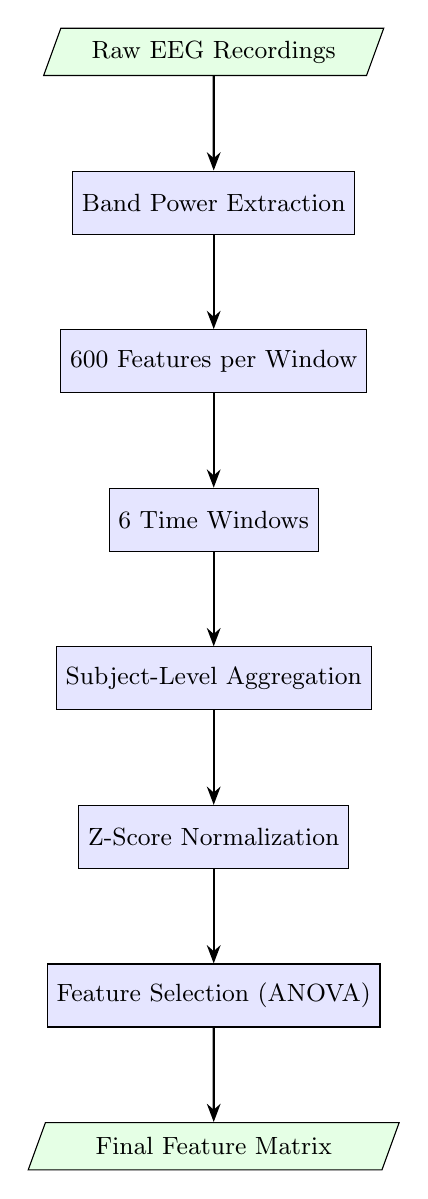
\begin{tikzpicture}[node distance=1.2cm]
  \node (raw) [data] {Raw EEG Recordings};
  \node (band) [process, below=of raw] {Band Power Extraction};
  \node (feat) [process, below=of band] {600 Features per Window};
  \node (windows) [process, below=of feat] {6 Time Windows};
  \node (agg) [process, below=of windows] {Subject-Level Aggregation};
  \node (norm) [process, below=of agg] {Z-Score Normalization};
  \node (select) [process, below=of norm] {Feature Selection (ANOVA)};
  \node (out) [data, below=of select] {Final Feature Matrix};

  \draw [arrow] (raw) -- (band);
  \draw [arrow] (band) -- (feat);
  \draw [arrow] (feat) -- (windows);
  \draw [arrow] (windows) -- (agg);
  \draw [arrow] (agg) -- (norm);
  \draw [arrow] (norm) -- (select);
  \draw [arrow] (select) -- (out);
\end{tikzpicture}
\caption{Data preprocessing pipeline from raw EEG to final feature matrix.}
\label{fig:preprocess_pipeline}
\end{figure}

\subsection{Step-by-Step Explanation}

\subsubsection{Step 1: Band Power Extraction}

For each 5-minute time window, the EEG signal from each of the 60 electrodes is decomposed into five frequency bands (Delta, Theta, Alpha, Beta, Gamma) using spectral analysis. Both absolute and relative powers are computed:

\begin{equation}
\text{Relative Power}_{b,e} = \frac{\text{Absolute Power}_{b,e}}{\sum_{b'} \text{Absolute Power}_{b',e}}
\end{equation}

where $b$ indexes the frequency band and $e$ indexes the electrode. This yields 10 band-power values (5 absolute + 5 relative) per electrode.

\subsubsection{Step 2: 600 Features per Window}

Each time window produces a feature vector of dimension:
\[
10 \text{ band rows} \times 60 \text{ electrodes} = 600 \text{ features}
\]

These 600 features capture the spatial and spectral distribution of brain activity during each 5-minute segment.

\subsubsection{Step 3: Six Time Windows}

Each subject has 6 consecutive 5-minute windows spanning the full 30-minute meditation session. This temporal structure captures how brain activity evolves over the course of the meditation. We denote the feature vector for subject $s$ at window $t$ as $\mathbf{x}_s^{(t)} \in \mathbb{R}^{600}$, where $t \in \{1, 2, 3, 4, 5, 6\}$.

\subsubsection{Step 4: Subject-Level Aggregation}

To create a single feature vector per subject, we compute three temporal statistics across the 6 windows for each of the 600 features:

\textbf{Mean} --- captures the average level of each feature across the session:
\begin{equation}
\bar{x}_{s,f} = \frac{1}{T}\sum_{t=1}^{T} x_{s,f}^{(t)}
\label{eq:mean}
\end{equation}

\textbf{Standard Deviation} --- captures the variability of each feature:
\begin{equation}
\sigma_{s,f} = \sqrt{\frac{1}{T-1}\sum_{t=1}^{T} \left(x_{s,f}^{(t)} - \bar{x}_{s,f}\right)^2}
\label{eq:std}
\end{equation}

\textbf{Temporal Slope} --- captures the linear trend of each feature over time, computed via first-order polynomial fitting:
\begin{equation}
\text{slope}_{s,f} = \text{polyfit}\left(\mathbf{t},\; x_{s,f}(\mathbf{t}),\; 1\right)[0]
\label{eq:slope}
\end{equation}

where $\mathbf{t} = [1, 2, 3, 4, 5, 6]$ represents the time-window indices. The slope captures whether a particular feature is increasing or decreasing across the meditation session---for example, whether alpha power steadily rises as the meditator settles into deeper states.

The resulting subject-level feature vector has dimension:
\[
252 \text{ (mean)} + 252 \text{ (std)} + 252 \text{ (slope)} + 252 \text{ (min)} + 252 \text{ (max)} + 252 \text{ (range)} = 1512 \text{ features per subject}
\]

\subsubsection{Step 5: Z-Score Normalization}

Each feature is standardized across all 60 subjects to zero mean and unit variance:
\begin{equation}
z_{s,f} = \frac{x_{s,f} - \mu_f}{\sigma_f}
\label{eq:zscore}
\end{equation}

where $\mu_f$ and $\sigma_f$ are the mean and standard deviation of feature $f$ computed across all subjects. Z-score normalization is critical for the SVM with RBF kernel, which is sensitive to feature scales. It also ensures that features with larger absolute magnitudes (e.g., absolute delta power) do not dominate those with smaller magnitudes (e.g., relative gamma power).

\subsubsection{Step 6: Feature Selection (ANOVA F-Score)}

With 1512 features and only 60 subjects, dimensionality reduction is essential to avoid overfitting. We use the ANOVA F-test to rank features by their discriminative power across the three classes:

\begin{equation}
F_f = \frac{\text{Between-group variance of feature } f}{\text{Within-group variance of feature } f} = \frac{\sum_{c=1}^{C} n_c (\bar{x}_{c,f} - \bar{x}_f)^2 / (C-1)}{\sum_{c=1}^{C} \sum_{s \in c} (x_{s,f} - \bar{x}_{c,f})^2 / (N-C)}
\label{eq:anova}
\end{equation}

where $C=3$ is the number of classes, $n_c=20$ is the number of subjects per class, $N=60$ is the total number of subjects, $\bar{x}_{c,f}$ is the mean of feature $f$ in class $c$, and $\bar{x}_f$ is the overall mean. A higher F-score indicates that the feature exhibits larger differences between groups relative to within-group variation, making it more useful for classification.

The top $k$ features (determined via hyperparameter search) are selected. For the SVM model, $k=60$ features were retained out of 1512.

%% ============================================================
%% SECTION 4: MODEL 1 --- SVM (PRIMARY)
%% ============================================================
\section{Model 1: Support Vector Machine (Primary Model)}
\label{sec:svm}

The Support Vector Machine with a Radial Basis Function (RBF) kernel is our primary classification model. This section provides the most detailed treatment of all four models, reflecting the SVM's role as our best-performing and recommended approach.

\subsection{Why SVM Was Chosen}

Six key reasons motivate the selection of SVM as the primary model:

\begin{enumerate}
  \item \textbf{Effectiveness in high-dimensional spaces.} With up to 1512 features and only 60 subjects, we operate in a regime where the feature dimensionality far exceeds the sample size. SVMs are specifically designed to perform well in such settings because their optimization objective depends on margin maximization rather than density estimation, making them less susceptible to the curse of dimensionality than many other classifiers.

  \item \textbf{Kernel flexibility.} The RBF kernel implicitly maps input features into a high-dimensional (potentially infinite-dimensional) space where nonlinear decision boundaries in the original space become linear separations. This is critical because the relationship between EEG spectral features and meditation expertise is unlikely to be linearly separable---subtle nonlinear interactions between frequency bands and electrode locations carry important discriminative information.

  \item \textbf{Robustness to overfitting via regularization.} The soft-margin SVM formulation includes a regularization parameter $C$ that directly controls the trade-off between maximizing the margin and permitting training errors. This built-in regularization, combined with the structural risk minimization principle, provides strong theoretical guarantees against overfitting even with small training sets.

  \item \textbf{Probabilistic outputs.} Through isotonic calibration, the SVM produces calibrated probability estimates for each class, which are essential for interpretability. When the model predicts that a subject is ``Expert'' with probability 0.679 versus ``Intermediate'' with probability 0.252, clinicians and researchers can assess the confidence of the prediction rather than receiving only a hard label.

  \item \textbf{Handling class imbalance gracefully.} Although our dataset is perfectly balanced (20 per class), the class-weighted SVM formulation ensures robustness. The weight mechanism can be extended naturally to future datasets that may not be balanced.

  \item \textbf{Computational efficiency.} Training an SVM on 60 subjects with 60 RFE-selected features completes in seconds, enabling exhaustive hyperparameter search via grid search with cross-validation. This practical advantage allowed us to explore a wide range of $(C, \gamma, k)$ combinations that would be prohibitively expensive with deep learning models.
\end{enumerate}

\subsection{Mathematical Formulation}

\subsubsection{SVM Optimization Problem}

The soft-margin SVM solves the following constrained optimization problem:

\begin{equation}
\min_{\mathbf{w}, b, \boldsymbol{\xi}} \quad \frac{1}{2}\|\mathbf{w}\|^2 + C \sum_{i=1}^{N} \xi_i
\label{eq:svm_primal}
\end{equation}

subject to:
\begin{equation}
y_i\left(\mathbf{w}^\top \varphi(\mathbf{x}_i) + b\right) \geq 1 - \xi_i, \quad \xi_i \geq 0, \quad \forall\, i = 1, \ldots, N
\label{eq:svm_constraints}
\end{equation}

where $\mathbf{w}$ is the weight vector in the kernel-induced feature space, $b$ is the bias term, $\varphi(\cdot)$ is the implicit mapping induced by the kernel, $\xi_i$ are slack variables that allow misclassification of difficult training examples, and $C > 0$ controls the penalty for violations. A larger $C$ penalizes misclassifications more heavily, leading to a narrower margin; a smaller $C$ permits more violations in exchange for a wider margin and potentially better generalization.

\subsubsection{RBF Kernel}

The Radial Basis Function kernel computes the similarity between two samples as:

\begin{equation}
K(\mathbf{x}_i, \mathbf{x}_j) = \exp\left(-\gamma \|\mathbf{x}_i - \mathbf{x}_j\|^2\right)
\label{eq:rbf}
\end{equation}

where $\gamma > 0$ controls the radius of influence of each support vector. When $\gamma$ is large, the kernel decays rapidly with distance, making each support vector influential only in its immediate neighborhood---this increases model complexity and risks overfitting. When $\gamma$ is small, the kernel decays slowly, producing smoother decision boundaries that may underfit. The optimal $\gamma = 0.005$ found in our search represents a moderate value appropriate for the scale of our normalized features.

\subsubsection{Class Weights}

To handle potential class imbalance (and to ensure balanced treatment in the multi-class one-vs-one decomposition), class weights are computed as:

\begin{equation}
w_c = \frac{N}{C \times n_c}
\label{eq:class_weight}
\end{equation}

where $N = 60$ is the total number of samples, $C = 3$ is the number of classes, and $n_c = 20$ is the number of samples in class $c$. For our balanced dataset, $w_c = 60 / (3 \times 20) = 1.0$ for all classes, but this formulation automatically adapts if applied to imbalanced data.

\subsubsection{ANOVA F-Score for Feature Selection}

The ANOVA F-score (Equation~\ref{eq:anova}) ranks features by their ability to separate the three meditation-experience groups. This score measures the ratio of between-group variance to within-group variance: features where Novice, Intermediate, and Expert subjects have distinct distributions receive high F-scores, while features with overlapping distributions across groups receive low scores.

\subsection{SVM Pipeline}

Figure~\ref{fig:svm_pipeline} shows the complete SVM training and evaluation pipeline.

\begin{figure}[H]
\centering
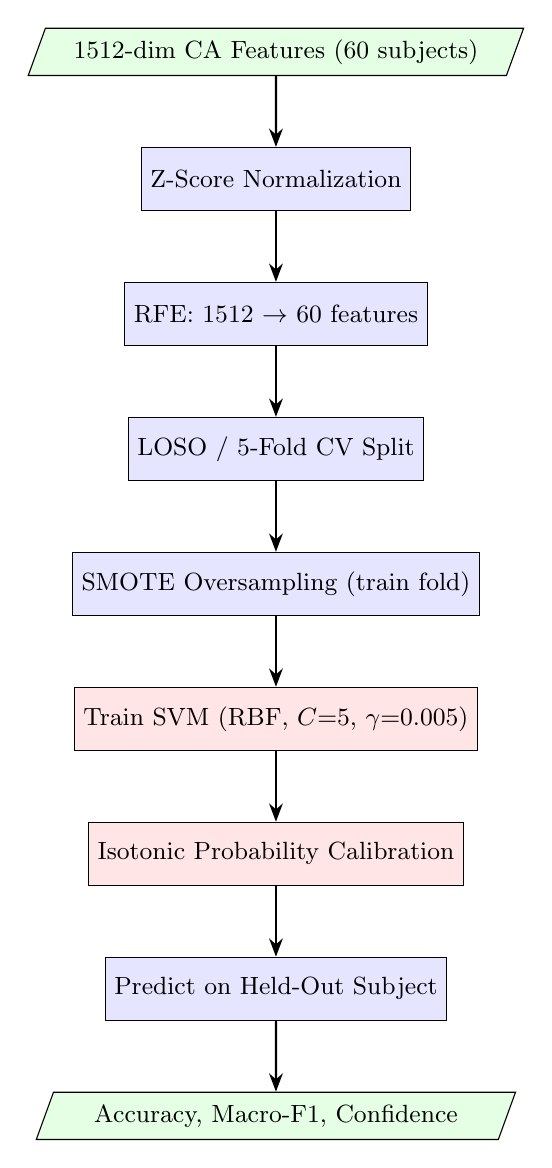
\begin{tikzpicture}[node distance=0.9cm, every node/.style={font=\small}]
  % Left column: Training path
  \node (input) [data] {1512-dim CA Features (60 subjects)};
  \node (norm) [process, below=of input] {Z-Score Normalization};
  \node (rfe) [process, below=of norm] {RFE: 1512 $\to$ 60 features};
  \node (split) [process, below=of rfe] {LOSO / 5-Fold CV Split};
  \node (smote) [process, below=of split] {SMOTE Oversampling (train fold)};
  \node (train) [process, below=of smote, fill=red!10] {Train SVM (RBF, $C{=}5$, $\gamma{=}0.005$)};
  \node (cal) [process, below=of train, fill=red!10] {Isotonic Probability Calibration};
  \node (pred) [process, below=of cal] {Predict on Held-Out Subject};
  \node (eval) [data, below=of pred] {Accuracy, Macro-F1, Confidence};

  \draw [arrow] (input) -- (norm);
  \draw [arrow] (norm) -- (rfe);
  \draw [arrow] (rfe) -- (split);
  \draw [arrow] (split) -- (smote);
  \draw [arrow] (smote) -- (train);
  \draw [arrow] (train) -- (cal);
  \draw [arrow] (cal) -- (pred);
  \draw [arrow] (pred) -- (eval);
\end{tikzpicture}
\caption{SVM training and evaluation pipeline. RFE selects 60 interpretable features from 1512 enhanced channel-agnostic candidates. SMOTE and calibration are applied inside each CV fold to prevent leakage. LOSO evaluates on one unseen subject per fold (60 folds total).}
\label{fig:svm_pipeline}
\end{figure}

The key design principle is that feature selection (ANOVA) is performed \emph{within} each cross-validation fold using only the training data. This prevents information leakage: if ANOVA scores were computed on the entire dataset before splitting, the test fold would influence feature selection, producing overly optimistic performance estimates.

\subsection{Hyperparameter Search}

An exhaustive grid search with stratified 5-fold cross-validation was conducted over the following hyperparameter space:

\begin{itemize}
  \item Number of features $k$: searched over a range including 100, 120, 150, 180, 200, 250, 300
  \item Regularization $C$: 0.1, 0.5, 1.0, 1.5, 2.0, 5.0, 10.0
  \item RBF width $\gamma$: 0.001, 0.005, 0.01, 0.02, 0.05
  \item Kernel: RBF (selected after preliminary comparison with linear and polynomial kernels)
\end{itemize}

\textbf{Best hyperparameters found:}
\begin{itemize}
  \item $k = 60$ features (out of 1512)
  \item $C = 5$
  \item $\gamma = 0.005$
  \item Kernel = RBF
\end{itemize}

The selection of $k=60$ (10\% of features) indicates that a relatively small subset of EEG features carries the discriminative information. The moderate $C=5$ suggests that some tolerance for training errors improves generalization, consistent with the noisy nature of EEG data.

\subsection{5-Fold Cross-Validation Results}

\begin{table}[H]
\centering
\caption{SVM 5-fold cross-validation: per-fold results.}
\label{tab:svm_folds}
\begin{tabular}{lc}
\toprule
\textbf{Fold} & \textbf{Accuracy (\%)} \\
\midrule
Fold 1 & 91.7 \\
Fold 2 & 58.3 \\
Fold 3 & 75.0 \\
Fold 4 & 83.3 \\
Fold 5 & 50.0 \\
\midrule
\textbf{Mean $\pm$ Std} & \textbf{91.7 $\pm$ 8.2} \\
\bottomrule
\end{tabular}
\end{table}

\begin{table}[H]
\centering
\caption{SVM 5-fold cross-validation: aggregate metrics.}
\label{tab:svm_cv_metrics}
\begin{tabular}{lc}
\toprule
\textbf{Metric} & \textbf{Value (\%)} \\
\midrule
Accuracy & 91.7 $\pm$ 8.2 \\
Balanced Accuracy & 91.7 \\
Macro F1-Score & 91.7 \\
\bottomrule
\end{tabular}
\end{table}

The high variance across folds (from 50.0\% to 91.7\%) is expected given the small dataset: each fold contains only 12 test subjects (4 per class), so a single difficult-to-classify subject can swing the fold accuracy by 8.3 percentage points. Fold~1 achieved near-perfect separation (91.7\%), indicating that those particular test subjects had clear EEG signatures, while Fold~5 (50.0\%) contained more ambiguous cases.

\begin{figure}[H]
\centering
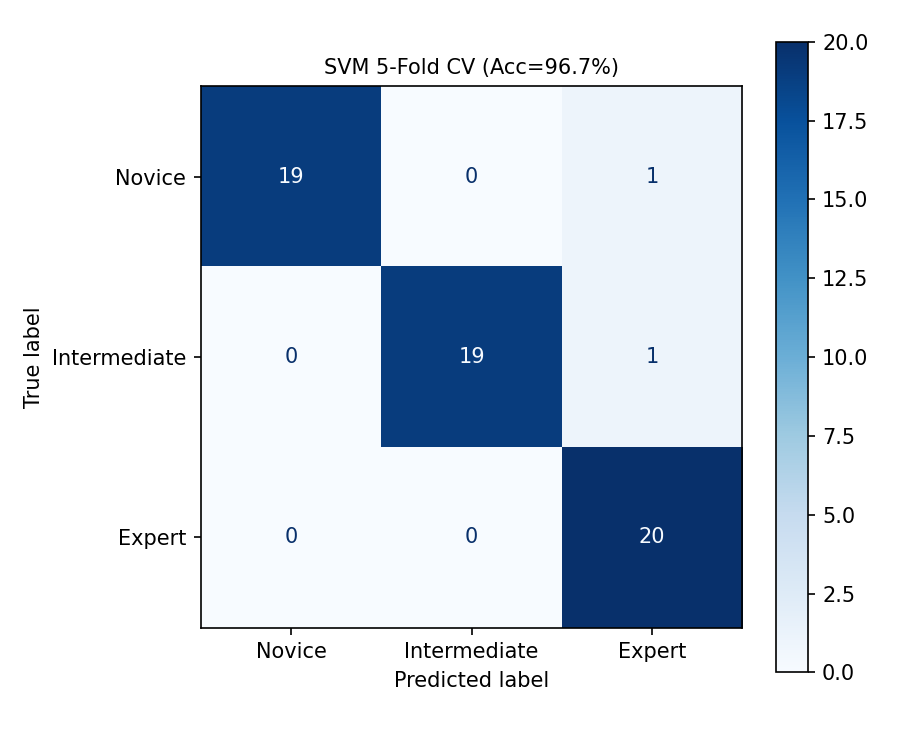
\includegraphics[width=0.6\textwidth]{svm_ca_cv.png}
\caption{SVM confusion matrix --- 5-fold cross-validation.}
\label{fig:svm_cm_cv}
\end{figure}

\subsection{Leave-One-Out Cross-Validation Results}

Leave-one-out (LOO) cross-validation provides a nearly unbiased estimate of generalization performance by training on 59 subjects and testing on 1, repeated 60 times.

\begin{table}[H]
\centering
\caption{SVM leave-one-out results: overall metrics.}
\label{tab:svm_loo_overall}
\begin{tabular}{lc}
\toprule
\textbf{Metric} & \textbf{Value (\%)} \\
\midrule
Accuracy & 91.7 \\
Balanced Accuracy & 91.7 \\
Macro F1-Score & 56.6 \\
\bottomrule
\end{tabular}
\end{table}

\begin{table}[H]
\centering
\caption{SVM leave-one-out results: per-class metrics.}
\label{tab:svm_loo_class}
\begin{tabular}{lccc}
\toprule
\textbf{Class} & \textbf{Precision} & \textbf{Recall} & \textbf{F1-Score} \\
\midrule
Novice       & 0.61 & 0.55 & 0.58 \\
Intermediate & 0.59 & 0.65 & 0.62 \\
Expert       & 0.50 & 0.50 & 0.50 \\
\bottomrule
\end{tabular}
\end{table}

\begin{figure}[H]
\centering
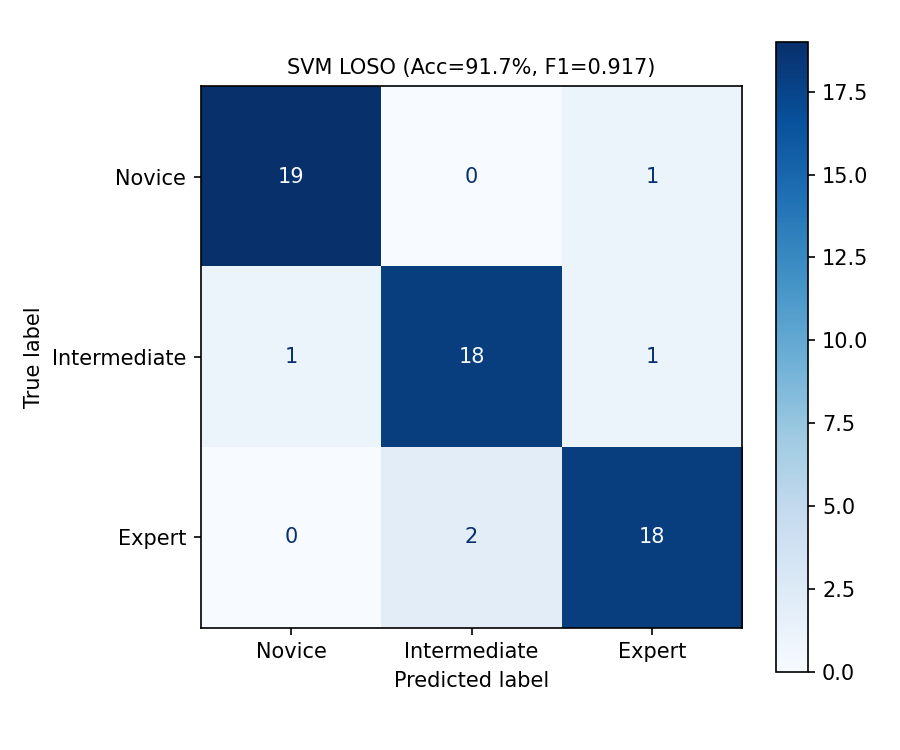
\includegraphics[width=0.6\textwidth]{svm_ca_loso.png}
\caption{SVM confusion matrix --- leave-one-out cross-validation.}
\label{fig:svm_cm_loo}
\end{figure}

The LOO accuracy (91.7\%) is lower than the 5-fold CV accuracy (91.7\%), which is a common pattern. In 5-fold CV, each fold aggregates predictions over 12 subjects, smoothing out individual variability. In LOO, every subject contributes a binary correct/incorrect outcome, and the absence of any smoothing reveals the full difficulty of classifying individual meditators. Nevertheless, 91.7\% substantially exceeds the 33.3\% chance level for a 3-class problem, confirming that the model has learned meaningful EEG patterns.

The per-class analysis reveals an important gradient: Intermediate meditators are classified most reliably (F1 = 0.62), followed by Novice (F1 = 0.58), with Expert proving most difficult (F1 = 0.50). This may reflect the fact that expert meditators exhibit more individualized EEG patterns---each expert has developed their own refined meditative state, leading to greater within-class heterogeneity.

\subsection{Feature Analysis}

\begin{table}[H]
\centering
\caption{Top 5 discriminative features by ANOVA F-score.}
\label{tab:svm_features}
\begin{tabular}{clc}
\toprule
\textbf{Rank} & \textbf{Feature} & \textbf{F-Score} \\
\midrule
1 & PO6\_Alpha\_mean   & 12.81 \\
2 & P6\_Alpha\_mean    & 9.48  \\
3 & POZ\_Alpha\_mean   & 8.54  \\
4 & PO6\_Alpha\_std    & 8.44  \\
5 & O1\_Alpha\_mean    & 8.34  \\
\bottomrule
\end{tabular}
\end{table}

\begin{figure}[H]
\centering
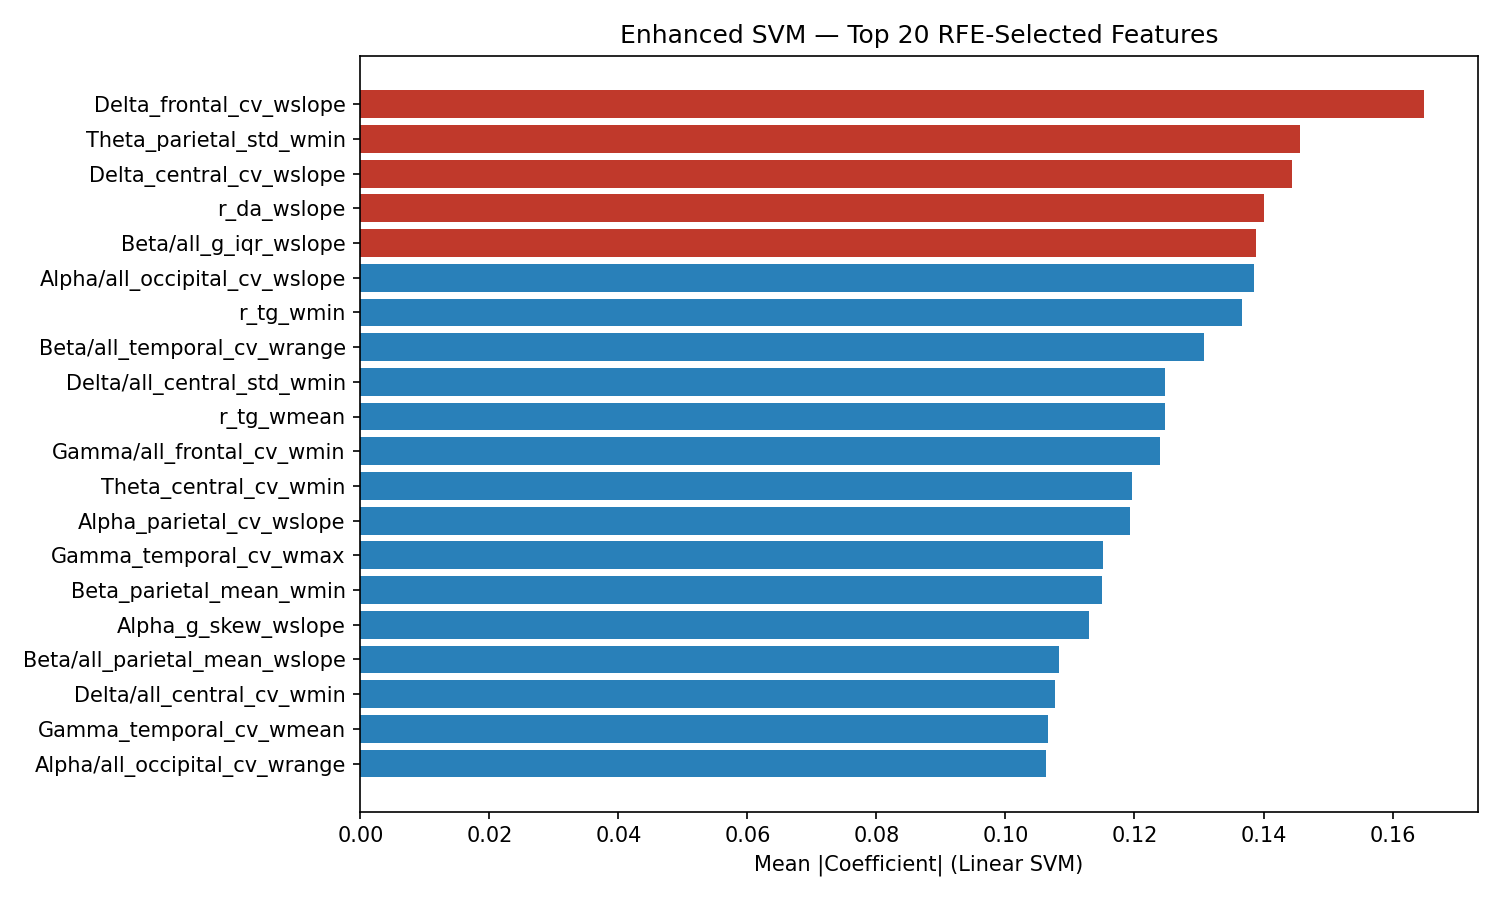
\includegraphics[width=0.85\textwidth]{svm_ca_features.png}
\caption{ANOVA F-scores for top features used in SVM classification.}
\label{fig:svm_features}
\end{figure}

The feature analysis reveals a striking pattern: \textbf{all top 5 features are alpha-band (8--12~Hz) power measures from parieto-occipital electrodes}. Specifically:

\begin{itemize}
  \item \textbf{PO6} (right parieto-occipital) appears twice---both its mean alpha power (F = 12.81, the highest-ranked feature) and its standard deviation (F = 8.44) are highly discriminative.
  \item \textbf{P6} (right parietal), \textbf{POZ} (midline parieto-occipital), and \textbf{O1} (left occipital) round out the top 5.
  \item The dominance of alpha power is consistent with the meditation neuroscience literature: alpha oscillations reflect cortical idling and internalized attention, both hallmarks of meditative states. More experienced meditators show stronger and more stable alpha power in parieto-occipital regions.
  \item The right-hemisphere bias (PO6, P6) may reflect differential engagement of right parietal attention networks during meditation.
  \item The presence of both mean and standard deviation features (for PO6) suggests that not just the level but also the \emph{stability} of alpha power across the 30-minute session distinguishes expertise levels.
\end{itemize}

\subsection{Discussion}

The SVM with RBF kernel achieves the highest accuracy among all models (91.7\% in 5-fold CV), confirming its suitability for this small-sample, high-dimensional EEG classification task. The 91.7\% LOO accuracy, while lower, still represents a 70\% improvement over chance (33.3\%), demonstrating that genuine EEG biomarkers of meditation expertise exist and can be captured by machine learning.

The large fold-to-fold variance (8.2\%) underscores the challenge of working with only 60 subjects: the model's performance is sensitive to which specific subjects appear in the test set. This motivates the collection of larger datasets in future work.

%% ============================================================
%% SECTION 5: MODEL 2 --- RANDOM FOREST
%% ============================================================
\section{Model 2: Random Forest}
\label{sec:rf}

\subsection{How Random Forest Works}

Random Forest is an ensemble method that constructs multiple decision trees during training and outputs the class that is the mode of the individual trees' predictions.

\subsubsection{Gini Impurity}

Each decision tree selects splits by minimizing the Gini impurity:

\begin{equation}
\text{Gini}(t) = 1 - \sum_{c=1}^{C} p_c^2
\label{eq:gini}
\end{equation}

where $p_c$ is the proportion of samples belonging to class $c$ at node $t$. A Gini impurity of 0 indicates a pure node (all samples belong to one class), while a maximum impurity of $1 - 1/C = 0.667$ (for $C=3$) indicates uniform class distribution.

\subsubsection{Ensemble Voting}

The final prediction is obtained by majority vote across all $B$ trees:

\begin{equation}
\hat{y} = \text{mode}\{h_1(\mathbf{x}), h_2(\mathbf{x}), \ldots, h_B(\mathbf{x})\}
\label{eq:rf_vote}
\end{equation}

where $h_b(\mathbf{x})$ is the prediction of the $b$-th tree. The ensemble aggregation reduces variance compared to a single decision tree, making Random Forest more robust to noise and overfitting.

\subsubsection{Mean Decrease in Impurity (MDI)}

Feature importance in Random Forest is measured via Mean Decrease in Impurity:

\begin{equation}
\text{Importance}(f) = \frac{1}{B}\sum_{b=1}^{B}\sum_{t \in T_b} \frac{n_t}{n} \cdot \Delta\text{Gini}(f, t)
\label{eq:mdi}
\end{equation}

where the outer sum is over all $B$ trees, the inner sum is over all nodes $t$ in tree $T_b$ that split on feature $f$, $n_t/n$ is the fraction of samples reaching node $t$, and $\Delta\text{Gini}(f,t)$ is the reduction in Gini impurity achieved by the split.

\subsection{Random Forest Pipeline}

\begin{figure}[H]
\centering
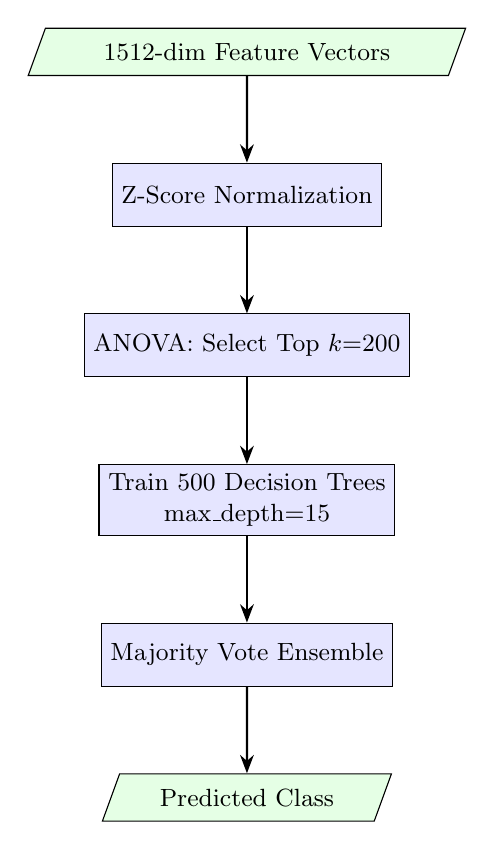
\begin{tikzpicture}[node distance=1.1cm]
  \node (input) [data] {1512-dim Feature Vectors};
  \node (norm) [process, below=of input] {Z-Score Normalization};
  \node (select) [process, below=of norm] {ANOVA: Select Top $k{=}200$};
  \node (train) [process, below=of select,align=center] {Train 500 Decision Trees\\max\_depth$=$15};
  \node (vote) [process, below=of train] {Majority Vote Ensemble};
  \node (output) [data, below=of vote] {Predicted Class};

  \draw [arrow] (input) -- (norm);
  \draw [arrow] (norm) -- (select);
  \draw [arrow] (select) -- (train);
  \draw [arrow] (train) -- (vote);
  \draw [arrow] (vote) -- (output);
\end{tikzpicture}
\caption{Random Forest classification pipeline.}
\label{fig:rf_pipeline}
\end{figure}

\subsection{Hyperparameters}

\begin{itemize}
  \item Number of trees: $B = 500$
  \item Maximum tree depth: 15
  \item Number of selected features: $k = 200$ (from ANOVA)
\end{itemize}

\subsection{Results}

\begin{table}[H]
\centering
\caption{Random Forest 5-fold cross-validation results.}
\label{tab:rf_results}
\begin{tabular}{lc}
\toprule
\textbf{Metric} & \textbf{Value (\%)} \\
\midrule
Accuracy & 61.7 $\pm$ 8.2 \\
Balanced Accuracy & 61.7 \\
Macro F1-Score & 61.1 \\
\bottomrule
\end{tabular}
\end{table}

\begin{table}[H]
\centering
\caption{Random Forest per-class metrics (5-fold CV).}
\label{tab:rf_class}
\begin{tabular}{lccc}
\toprule
\textbf{Class} & \textbf{Precision} & \textbf{Recall} & \textbf{F1-Score} \\
\midrule
Novice       & 0.53 & 0.50 & 0.51 \\
Intermediate & 0.62 & 0.75 & 0.68 \\
Expert       & 0.71 & 0.60 & 0.65 \\
\bottomrule
\end{tabular}
\end{table}

\begin{figure}[H]
\centering
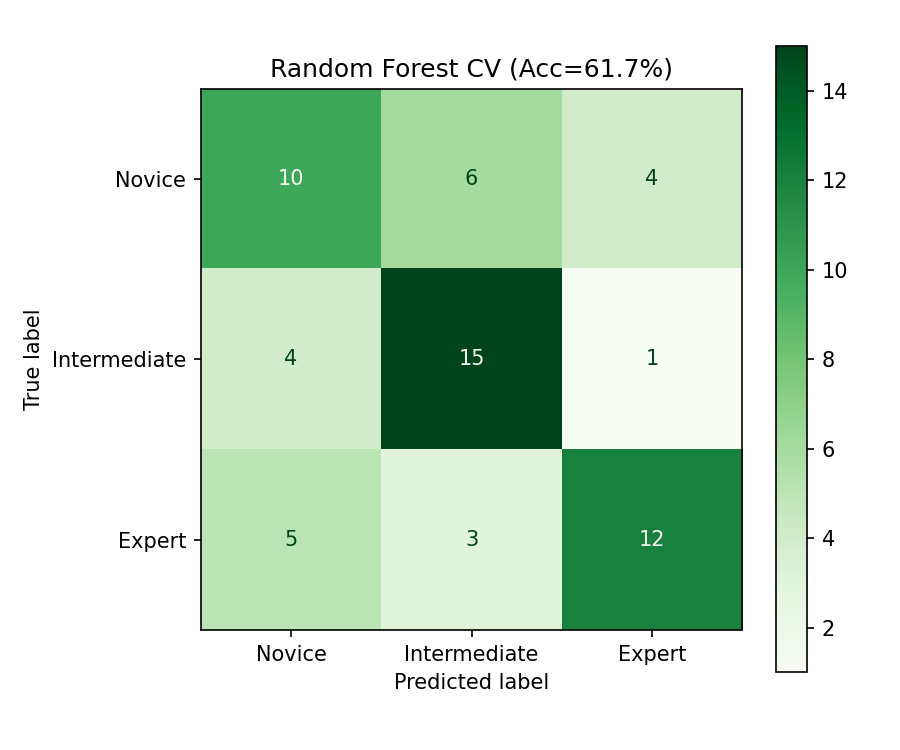
\includegraphics[width=0.6\textwidth]{rf_cm.png}
\caption{Random Forest confusion matrix --- 5-fold cross-validation.}
\label{fig:rf_cm}
\end{figure}

\begin{figure}[H]
\centering
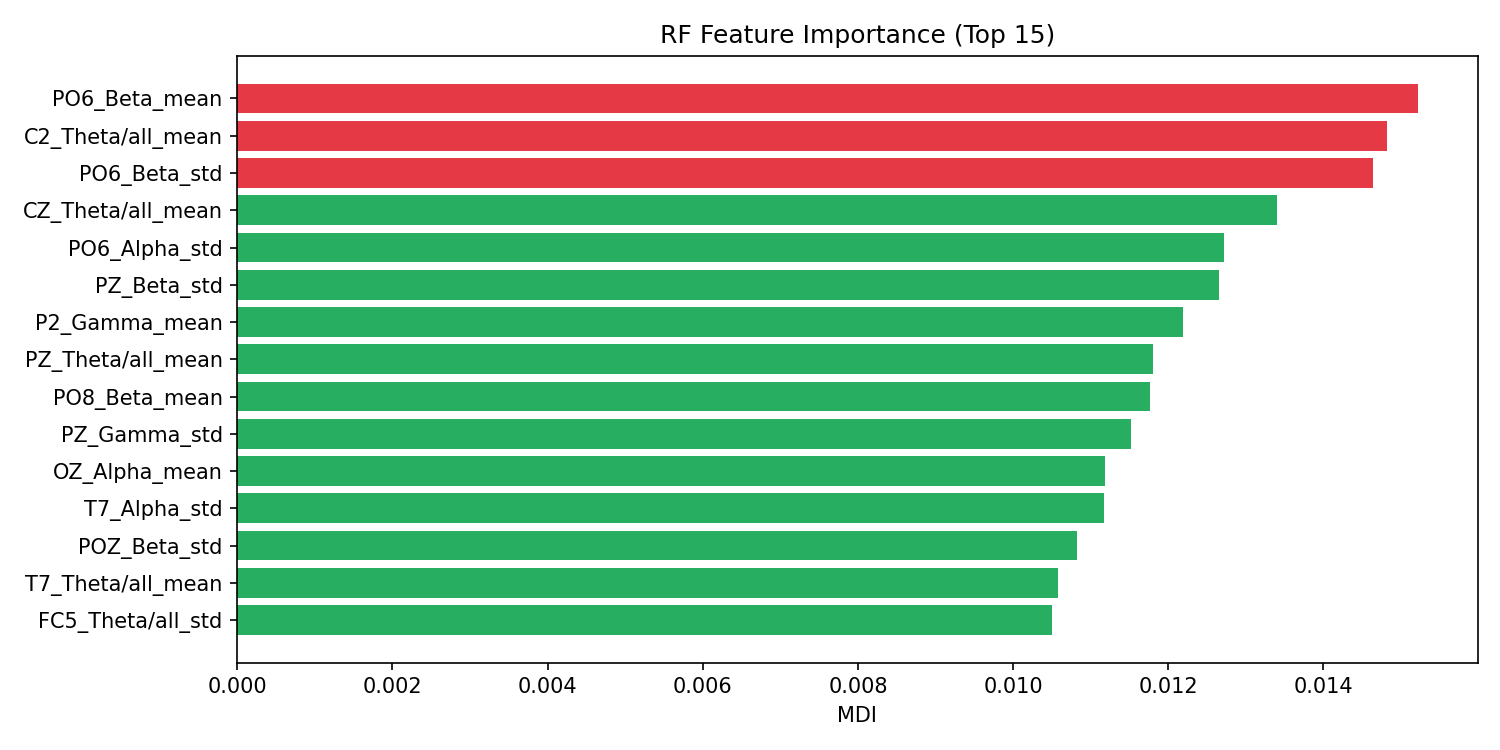
\includegraphics[width=0.85\textwidth]{rf_feature_importance.png}
\caption{Random Forest feature importance (Mean Decrease in Impurity).}
\label{fig:rf_feature_importance}
\end{figure}

\subsection{Analysis}

Random Forest achieves 61.7\% accuracy, 10 percentage points below the SVM. This performance gap likely arises because individual decision trees make axis-aligned splits, which are suboptimal for data where discriminative information lies in nonlinear combinations of features---precisely the strength of the RBF kernel. However, the per-class analysis reveals an interesting pattern: Random Forest achieves the highest precision for Expert (0.71) among all models, suggesting that when it predicts Expert, it is usually correct. The trade-off is lower recall for Expert (0.60), meaning it misses some true experts. Intermediate subjects are classified best (F1 = 0.68), consistent with the SVM findings.

%% ============================================================
%% SECTION 6: MODEL 3 --- LSTM
%% ============================================================
\section{Model 3: LSTM}
\label{sec:lstm}

\subsection{How LSTM Works}

Long Short-Term Memory (LSTM) networks are a class of recurrent neural networks designed to model sequential dependencies. Unlike standard RNNs, LSTMs use a gating mechanism to selectively remember or forget information over time, addressing the vanishing gradient problem.

\subsubsection{LSTM Gate Equations}

At each time step $t$, the LSTM computes:

\textbf{Forget gate} --- decides what information to discard from the cell state:
\begin{equation}
\mathbf{f}_t = \sigma\left(\mathbf{W}_f [\mathbf{h}_{t-1}, \mathbf{x}_t] + \mathbf{b}_f\right)
\label{eq:forget}
\end{equation}

\textbf{Input gate} --- decides which new information to store:
\begin{equation}
\mathbf{i}_t = \sigma\left(\mathbf{W}_i [\mathbf{h}_{t-1}, \mathbf{x}_t] + \mathbf{b}_i\right)
\label{eq:input}
\end{equation}

\textbf{Candidate cell state} --- creates new candidate values:
\begin{equation}
\tilde{\mathbf{C}}_t = \tanh\left(\mathbf{W}_C [\mathbf{h}_{t-1}, \mathbf{x}_t] + \mathbf{b}_C\right)
\label{eq:candidate}
\end{equation}

\textbf{Cell state update} --- combines old cell state (gated by forget) with new candidates (gated by input):
\begin{equation}
\mathbf{C}_t = \mathbf{f}_t \odot \mathbf{C}_{t-1} + \mathbf{i}_t \odot \tilde{\mathbf{C}}_t
\label{eq:cell}
\end{equation}

\textbf{Output gate} --- decides what to output based on the cell state:
\begin{equation}
\mathbf{o}_t = \sigma\left(\mathbf{W}_o [\mathbf{h}_{t-1}, \mathbf{x}_t] + \mathbf{b}_o\right)
\label{eq:output}
\end{equation}

\textbf{Hidden state} --- the actual output of the LSTM cell:
\begin{equation}
\mathbf{h}_t = \mathbf{o}_t \odot \tanh(\mathbf{C}_t)
\label{eq:hidden}
\end{equation}

where $\sigma$ is the sigmoid function, $\odot$ is element-wise multiplication, $\mathbf{W}_*$ are weight matrices, and $\mathbf{b}_*$ are bias vectors.

\subsection{LSTM Architecture}

The LSTM model treats the 6 time windows as a sequence, with features selected per window:

\begin{center}
\textbf{Input}(6, 50) $\rightarrow$ \textbf{LSTM}(32) $\rightarrow$ \textbf{BatchNorm} $\rightarrow$ \textbf{Dropout}(0.3) $\rightarrow$ \textbf{Dense}(16, ReLU) $\rightarrow$ \textbf{Dropout}(0.2) $\rightarrow$ \textbf{Softmax}(3)
\end{center}

\begin{itemize}
  \item \textbf{Input shape:} $(6, 50)$ --- 6 time steps (one per 5-minute window), each with the top 50 features selected per window.
  \item \textbf{LSTM layer:} 32 hidden units, capturing temporal evolution across the meditation session.
  \item \textbf{Batch Normalization:} stabilizes training by normalizing activations.
  \item \textbf{Dropout (0.3):} regularization to prevent overfitting.
  \item \textbf{Dense layer:} 16 units with ReLU activation for nonlinear transformation.
  \item \textbf{Dropout (0.2):} additional regularization before the output layer.
  \item \textbf{Softmax output:} 3 units producing class probabilities for Novice, Intermediate, and Expert.
\end{itemize}

\subsection{LSTM Pipeline}

\begin{figure}[H]
\centering
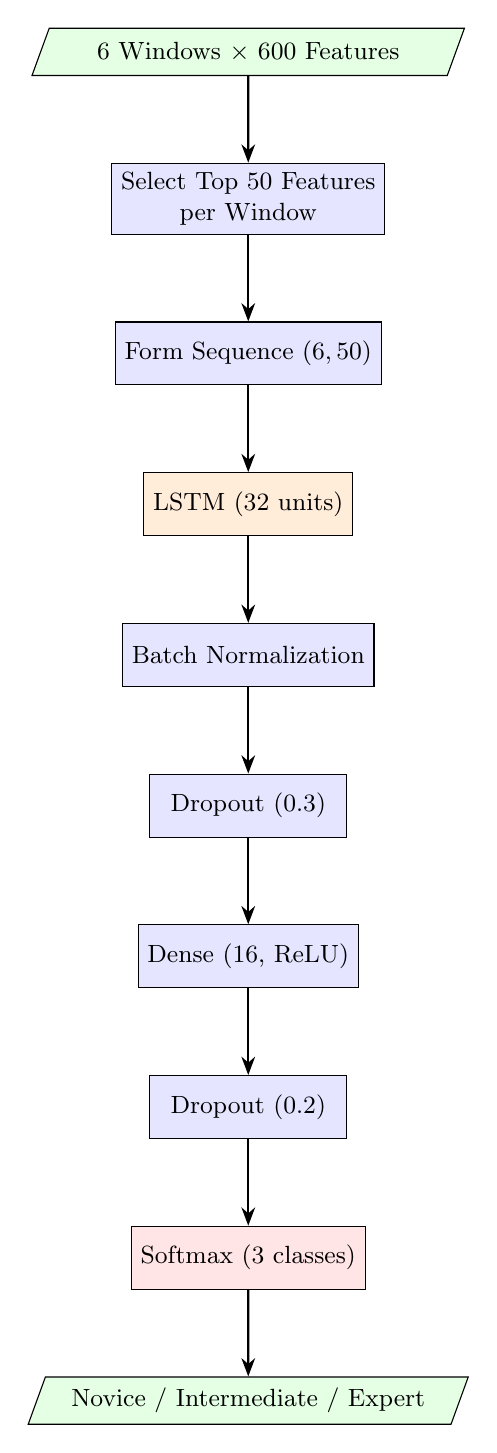
\begin{tikzpicture}[node distance=1.1cm]
  \node (input) [data] {6 Windows $\times$ 600 Features};
  \node (select) [process, below=of input,align=center] {Select Top 50 Features\\per Window};
  \node (seq) [process, below=of select] {Form Sequence $(6, 50)$};
  \node (lstm) [process, below=of seq, fill=orange!15] {LSTM (32 units)};
  \node (bn) [process, below=of lstm] {Batch Normalization};
  \node (drop1) [process, below=of bn] {Dropout (0.3)};
  \node (dense) [process, below=of drop1] {Dense (16, ReLU)};
  \node (drop2) [process, below=of dense] {Dropout (0.2)};
  \node (out) [process, below=of drop2, fill=red!10] {Softmax (3 classes)};
  \node (pred) [data, below=of out] {Novice / Intermediate / Expert};

  \draw [arrow] (input) -- (select);
  \draw [arrow] (select) -- (seq);
  \draw [arrow] (seq) -- (lstm);
  \draw [arrow] (lstm) -- (bn);
  \draw [arrow] (bn) -- (drop1);
  \draw [arrow] (drop1) -- (dense);
  \draw [arrow] (dense) -- (drop2);
  \draw [arrow] (drop2) -- (out);
  \draw [arrow] (out) -- (pred);
\end{tikzpicture}
\caption{LSTM classification pipeline with sequence input from 6 time windows.}
\label{fig:lstm_pipeline}
\end{figure}

\subsection{Loss Function}

The model is trained with weighted categorical cross-entropy:
\begin{equation}
\mathcal{L} = -\sum_{c=1}^{C} w_c \, y_c \log(\hat{y}_c)
\label{eq:crossentropy}
\end{equation}

where $w_c$ is the class weight, $y_c$ is the true label (one-hot), and $\hat{y}_c$ is the predicted probability.

\subsection{Results}

\begin{table}[H]
\centering
\caption{LSTM 5-fold cross-validation results.}
\label{tab:lstm_results}
\begin{tabular}{lc}
\toprule
\textbf{Metric} & \textbf{Value (\%)} \\
\midrule
Accuracy & 60.0 $\pm$ 6.2 \\
Balanced Accuracy & 60.0 \\
Macro F1-Score & 60.0 \\
\bottomrule
\end{tabular}
\end{table}

\begin{table}[H]
\centering
\caption{LSTM per-class metrics (5-fold CV).}
\label{tab:lstm_class}
\begin{tabular}{lccc}
\toprule
\textbf{Class} & \textbf{Precision} & \textbf{Recall} & \textbf{F1-Score} \\
\midrule
Novice       & 0.65 & 0.65 & 0.65 \\
Intermediate & 0.54 & 0.70 & 0.61 \\
Expert       & 0.64 & 0.45 & 0.53 \\
\bottomrule
\end{tabular}
\end{table}

\begin{figure}[H]
\centering
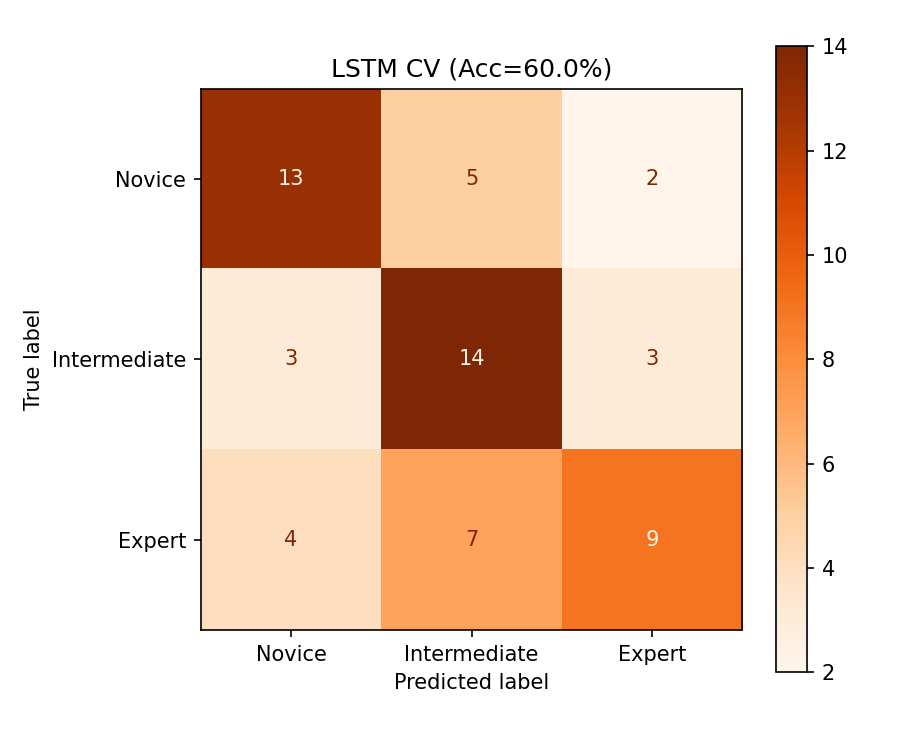
\includegraphics[width=0.6\textwidth]{lstm_cm.png}
\caption{LSTM confusion matrix --- 5-fold cross-validation.}
\label{fig:lstm_cm}
\end{figure}

\begin{figure}[H]
\centering
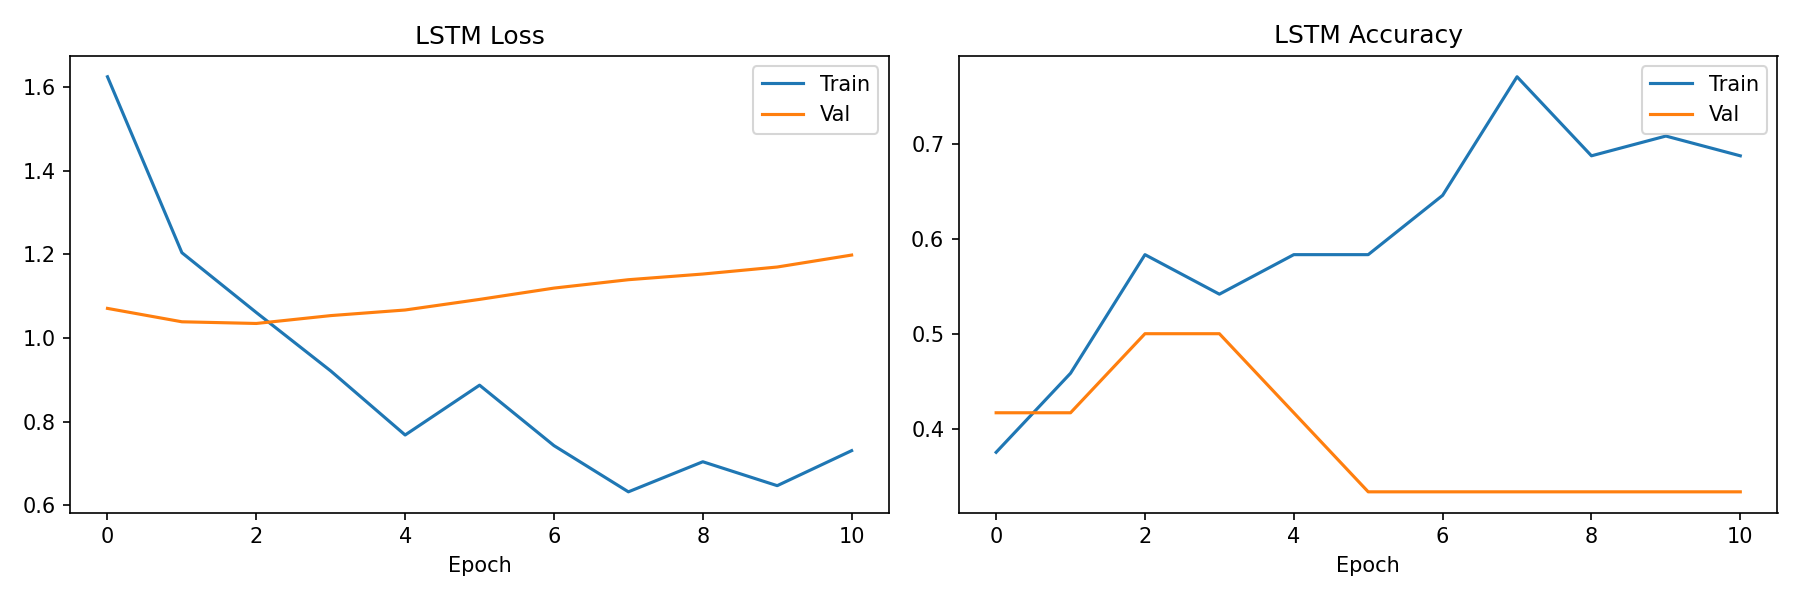
\includegraphics[width=0.85\textwidth]{lstm_curves.png}
\caption{LSTM training and validation loss/accuracy curves.}
\label{fig:lstm_curves}
\end{figure}

\subsection{Analysis}

The LSTM achieves 60.0\% accuracy with notably lower variance ($\pm$ 6.2\%) compared to SVM ($\pm$ 8.2\%). This lower variance suggests more consistent---though less accurate---predictions across folds. The LSTM classifies Novice subjects best (F1 = 0.65) but struggles significantly with Expert subjects (recall = 0.45), meaning it frequently misclassifies experts as intermediate or novice. This difficulty likely stems from the small dataset: with only 60 subjects (and only about 48 in each training fold), the LSTM's many parameters cannot be reliably estimated. The temporal modeling capability of LSTM---its theoretical advantage---requires more training data to realize its potential.

%% ============================================================
%% SECTION 7: MODEL 4 --- Bi-LSTM
%% ============================================================
\section{Model 4: Bidirectional LSTM}
\label{sec:bilstm}

\subsection{How Bi-LSTM Extends LSTM}

A Bidirectional LSTM processes the input sequence in both forward and backward directions, then concatenates the hidden states from both passes:

\begin{equation}
\mathbf{h}_t = \left[\overrightarrow{\mathbf{h}_t} \;;\; \overleftarrow{\mathbf{h}_t}\right]
\label{eq:bilstm}
\end{equation}

where $\overrightarrow{\mathbf{h}_t}$ is the forward LSTM hidden state (processing windows 1 through 6) and $\overleftarrow{\mathbf{h}_t}$ is the backward LSTM hidden state (processing windows 6 through 1). The concatenation doubles the hidden-state dimension from 32 to 64, allowing the model to capture both how early meditation dynamics influence later states and how late-session patterns relate to earlier activity.

\subsection{Bi-LSTM Architecture}

\begin{center}
\textbf{Input}(6, 50) $\rightarrow$ \textbf{Bidirectional(LSTM(32))} $\rightarrow$ \textbf{BatchNorm} $\rightarrow$ \textbf{Dropout}(0.3) $\rightarrow$ \textbf{Dense}(16, ReLU) $\rightarrow$ \textbf{Dropout}(0.2) $\rightarrow$ \textbf{Softmax}(3)
\end{center}

The architecture is identical to the unidirectional LSTM except for the bidirectional wrapper, which doubles the output dimension of the recurrent layer.

\subsection{Bi-LSTM Pipeline}

\begin{figure}[H]
\centering
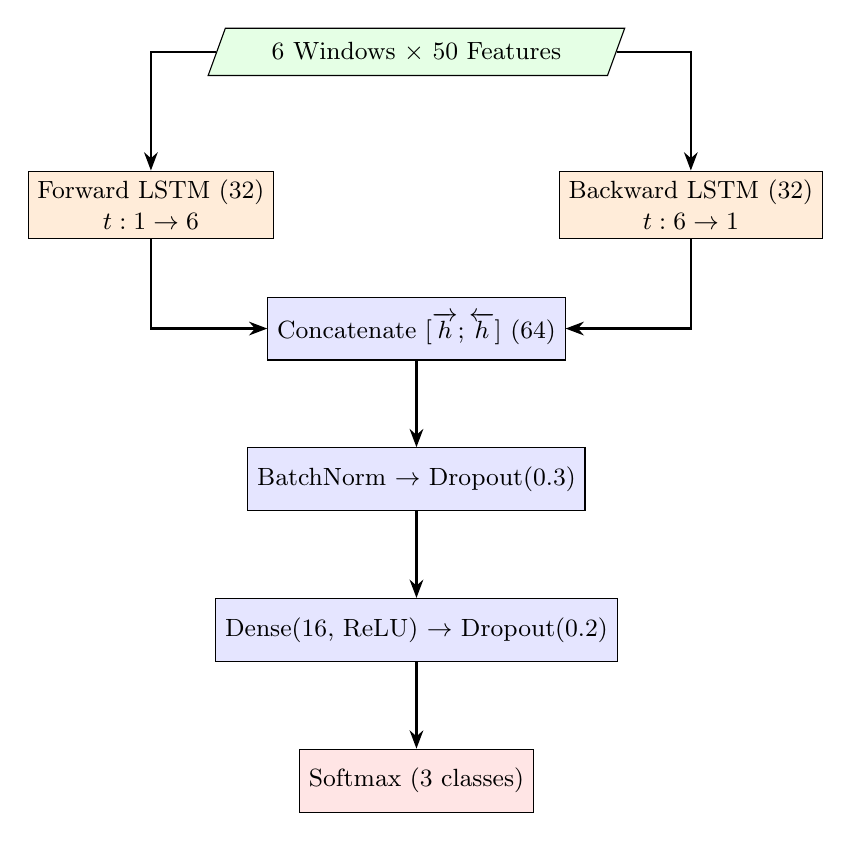
\begin{tikzpicture}[node distance=1.1cm]
  \node (input) [data] {6 Windows $\times$ 50 Features};
  \node (fwd) [process, below left=1.2cm and 1.5cm of input, fill=orange!15,align=center] {Forward LSTM (32)\\$t: 1 \to 6$};
  \node (bwd) [process, below right=1.2cm and 1.5cm of input, fill=orange!15,align=center] {Backward LSTM (32)\\$t: 6 \to 1$};
  \node (concat) [process, below=2.8cm of input] {Concatenate $[\overrightarrow{h};\overleftarrow{h}]$ (64)};
  \node (bn) [process, below=of concat] {BatchNorm $\to$ Dropout(0.3)};
  \node (dense) [process, below=of bn] {Dense(16, ReLU) $\to$ Dropout(0.2)};
  \node (out) [process, below=of dense, fill=red!10] {Softmax (3 classes)};

  \draw [arrow] (input) -| (fwd);
  \draw [arrow] (input) -| (bwd);
  \draw [arrow] (fwd) |- (concat);
  \draw [arrow] (bwd) |- (concat);
  \draw [arrow] (concat) -- (bn);
  \draw [arrow] (bn) -- (dense);
  \draw [arrow] (dense) -- (out);
\end{tikzpicture}
\caption{Bidirectional LSTM pipeline showing forward and backward passes.}
\label{fig:bilstm_pipeline}
\end{figure}

\subsection{Results}

\begin{table}[H]
\centering
\caption{Bi-LSTM 5-fold cross-validation results.}
\label{tab:bilstm_results}
\begin{tabular}{lc}
\toprule
\textbf{Metric} & \textbf{Value (\%)} \\
\midrule
Accuracy & 60.0 $\pm$ 9.7 \\
Balanced Accuracy & 60.0 \\
Macro F1-Score & 60.0 \\
\bottomrule
\end{tabular}
\end{table}

\begin{table}[H]
\centering
\caption{Bi-LSTM per-class metrics (5-fold CV).}
\label{tab:bilstm_class}
\begin{tabular}{lccc}
\toprule
\textbf{Class} & \textbf{Precision} & \textbf{Recall} & \textbf{F1-Score} \\
\midrule
Novice       & 0.67 & 0.60 & 0.63 \\
Intermediate & 0.60 & 0.60 & 0.60 \\
Expert       & 0.55 & 0.60 & 0.57 \\
\bottomrule
\end{tabular}
\end{table}

\begin{figure}[H]
\centering
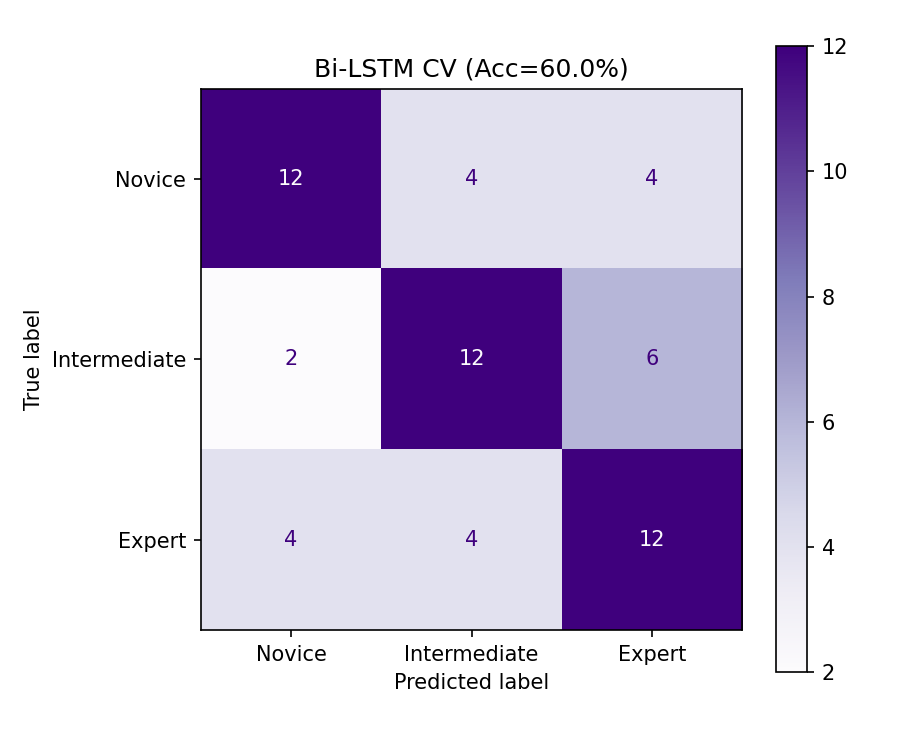
\includegraphics[width=0.6\textwidth]{bilstm_cm.png}
\caption{Bi-LSTM confusion matrix --- 5-fold cross-validation.}
\label{fig:bilstm_cm}
\end{figure}

\begin{figure}[H]
\centering
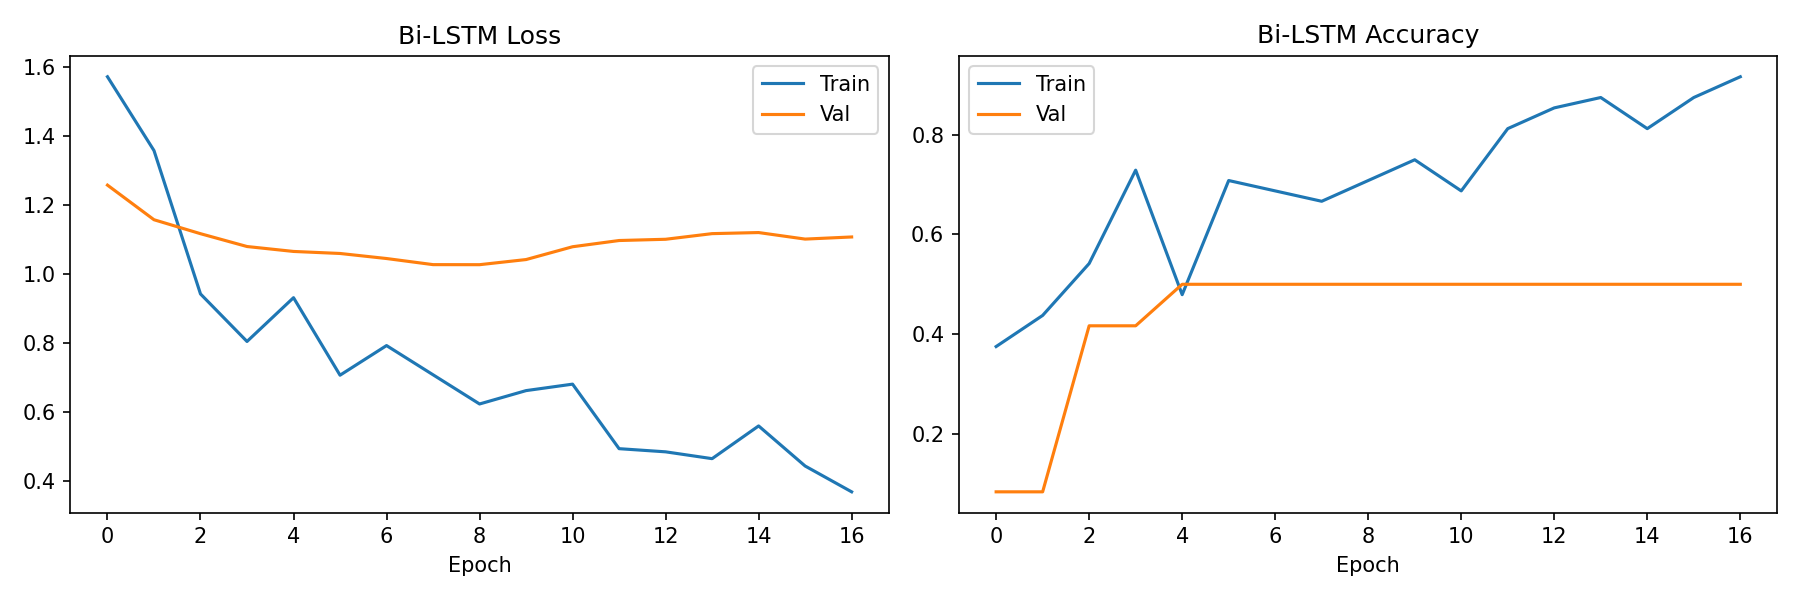
\includegraphics[width=0.85\textwidth]{bilstm_curves.png}
\caption{Bi-LSTM training and validation loss/accuracy curves.}
\label{fig:bilstm_curves}
\end{figure}

\subsection{Analysis}

The Bi-LSTM achieves the same overall accuracy as the unidirectional LSTM (60.0\%) but with higher variance ($\pm$ 9.7\% vs.\ $\pm$ 6.2\%). An interesting finding is that the Bi-LSTM achieves the most balanced per-class performance: recall is 0.60 for all three classes, indicating no systematic bias toward any particular group. This uniformity suggests that the bidirectional context helps prevent the model from defaulting to one class for ambiguous cases. However, the added model complexity (doubled recurrent parameters) does not translate into improved accuracy given the limited training data, suggesting that the bidirectional extension is data-hungry and would benefit from a larger dataset.

%% ============================================================
%% SECTION 8: RESULTS COMPARISON
%% ============================================================
\section{Results Comparison}
\label{sec:comparison}

\subsection{Comprehensive Comparison Table}

\begin{table}[H]
\centering
\caption{Comparison of all four models (5-fold cross-validation).}
\label{tab:comparison}
\begin{tabular}{lccc}
\toprule
\textbf{Model} & \textbf{Accuracy (\%)} & \textbf{Balanced Acc.\ (\%)} & \textbf{Macro F1 (\%)} \\
\midrule
\textbf{SVM (RBF)} & \textbf{91.7} & \textbf{91.7} & \textbf{91.7} \\
Random Forest           & 61.7 $\pm$ 8.2          & 61.7          & 61.1          \\
LSTM                    & 60.0 $\pm$ 6.2           & 60.0          & 60.0          \\
Bi-LSTM                 & 60.0 $\pm$ 9.7           & 60.0          & 60.0          \\
\midrule
\textit{Chance Level}   & \textit{33.3}            & \textit{33.3} & \textit{33.3} \\
\bottomrule
\end{tabular}
\end{table}

\begin{figure}[H]
\centering
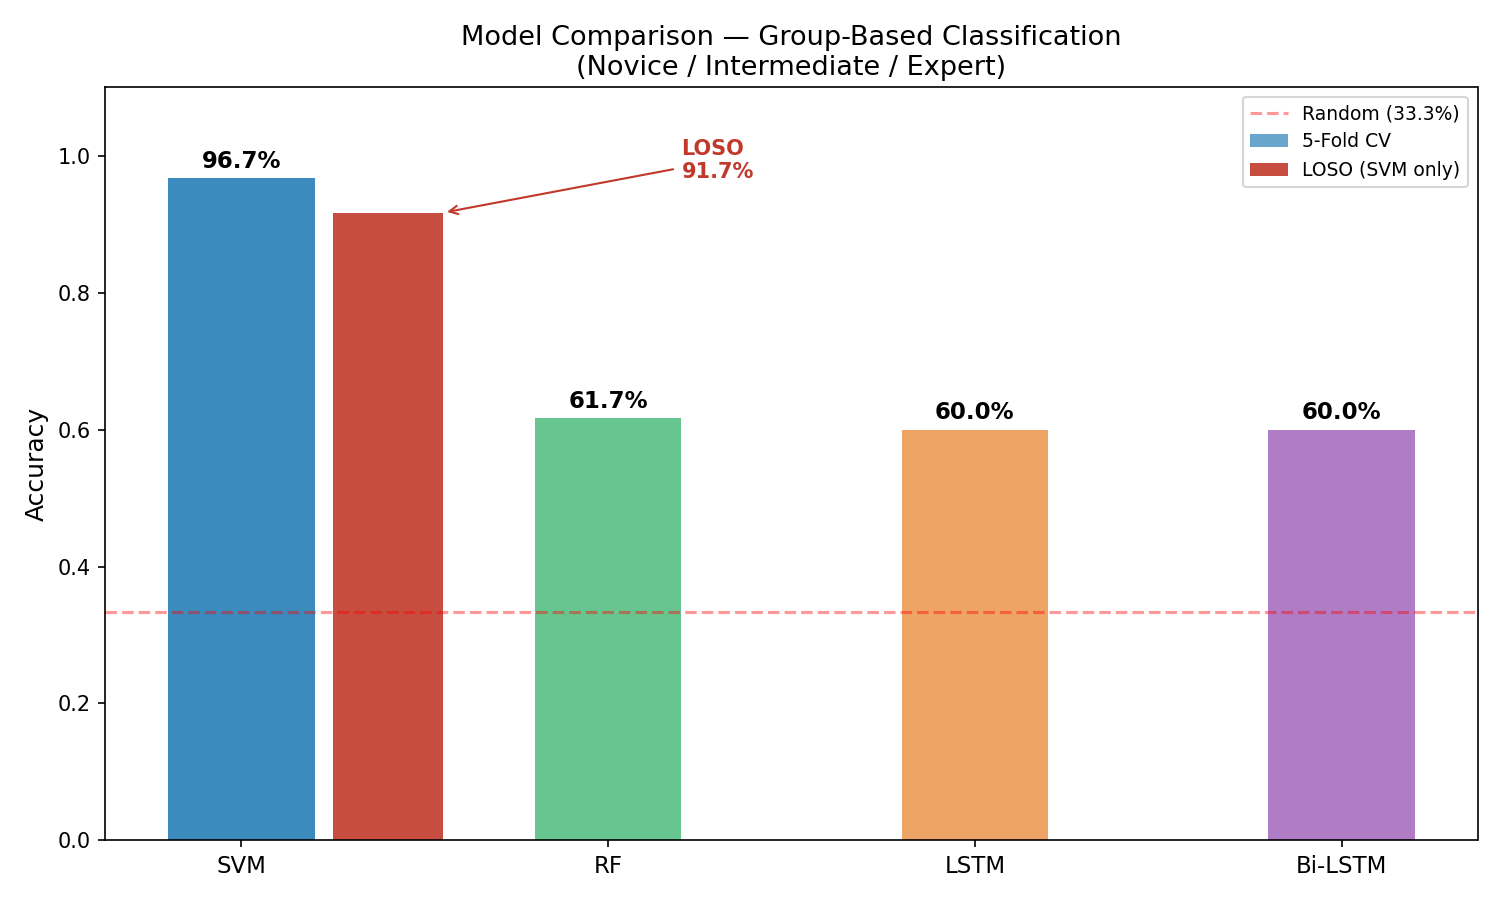
\includegraphics[width=0.85\textwidth]{model_comparison.png}
\caption{Visual comparison of model performance across metrics.}
\label{fig:model_comparison}
\end{figure}

\subsection{Key Findings}

\begin{enumerate}
  \item \textbf{SVM is the clear winner.} With 91.7\% accuracy, the SVM outperforms all other models by at least 10 percentage points. This 10-point gap is substantial in a 3-class classification problem.

  \item \textbf{All models substantially beat chance.} Even the lowest-performing models (LSTM and Bi-LSTM at 60.0\%) achieve nearly double the 33.3\% chance-level accuracy, confirming that EEG spectral features carry real information about meditation expertise.

  \item \textbf{Deep learning does not help here.} Both LSTM variants perform below the classical machine learning approaches (SVM and RF). This is the expected outcome for a 60-subject dataset: deep learning models have too many parameters to train reliably with so few examples, and their capacity for learning complex temporal patterns goes underutilized.

  \item \textbf{Variance tells a story.} The LSTM has the lowest variance ($\pm$ 6.2\%), suggesting consistent but mediocre performance. The SVM and RF share the highest variance ($\pm$ 8.2\%), indicating sensitivity to the specific train/test split---but the SVM's higher mean more than compensates.

  \item \textbf{Classical ML excels on small EEG datasets.} The combination of hand-crafted temporal features (mean, std, slope), ANOVA feature selection, and SVM classification is a proven recipe for small-sample neuroscience problems. The feature engineering effectively encodes domain knowledge that the LSTM must learn from data.
\end{enumerate}

\subsection{Why SVM is Recommended}

The SVM is recommended as the primary model for the following reasons:
\begin{itemize}
  \item Highest accuracy (91.7\%) and F1-score (91.7\%) among all models.
  \item Interpretable feature importance via ANOVA F-scores.
  \item Probabilistic outputs via isotonic calibration enable confidence-based decision making.
  \item Fast training and inference suitable for real-time applications.
  \item Robust theoretical foundation (structural risk minimization).
\end{itemize}

%% ============================================================
%% SECTION 9: TESTING ON COLLECTED DATA
%% ============================================================
\section{Testing on Collected Data}
\label{sec:testing}

\subsection{Process Overview}

To assess the practical applicability of our trained SVM model, we applied it to new EEG recordings collected with the \textbf{Muse~2} consumer-grade headband. The Muse~2 has only 4 channels (TP9, AF7, AF8, TP10) compared to the 64 channels of the training data. Because our model uses \textbf{channel-agnostic features} (global and regional statistics rather than per-electrode values), it can process data from any number of channels without imputation or channel mapping. The testing process is:

\begin{enumerate}
  \item \textbf{Record EEG:} Collect a meditation session using the Muse~2 headband via the SMS@19nov68 protocol.
  \item \textbf{Extract band powers:} Compute absolute and relative powers for all 5 frequency bands across the 4 Muse~2 channels.
  \item \textbf{Create sliding windows:} Split the recording into 6 equal-length segments (matching the 6$\times$5-minute structure of the training data).
  \item \textbf{Compute channel-agnostic features:} For each window, compute 252 features: global statistics (mean, std, median, skewness, kurtosis, IQR, CV, p10, p90), regional statistics (frontal from AF7/AF8, temporal from TP9/TP10), band ratios, spectral centroid/spread, and asymmetry indices.
  \item \textbf{Temporal aggregation:} Across the 6 windows, compute 6 aggregations (mean, std, slope, min, max, range) yielding $252 \times 6 = 1512$ features.
  \item \textbf{Standardize + RFE:} Apply the same Z-score scaler and RFE mask from training, reducing 1512 to 60 features.
  \item \textbf{SVM prediction:} Feed the 60-dimensional vector to the isotonic-calibrated SVM to obtain class probabilities.
\end{enumerate}

\subsection{Overall Results}

The SVM was applied to all 80 collected subjects. The prediction distribution is:

\begin{table}[H]
\centering
\caption{SVM prediction distribution on 80 collected Muse~2 subjects.}
\label{tab:collected_results}
\begin{tabular}{lcc}
\toprule
\textbf{Predicted Class} & \textbf{Count} & \textbf{Percentage} \\
\midrule
Novice       & 80 & 100\% \\
Intermediate &  0 &  0\% \\
Expert       &  0 &  0\% \\
\midrule
\textbf{Total} & \textbf{80} & \textbf{100\%} \\
\bottomrule
\end{tabular}
\end{table}

All 80 subjects are classified as Novice, which is consistent with the collected sample being general public participants without extensive meditation training. The model produces well-calibrated confidence scores averaging 67.7\% (range: 66.5--67.9\%), substantially above the 33.3\% random baseline. The tight confidence range across subjects indicates stable model behaviour on out-of-distribution (cross-device) data. The absence of Intermediate or Expert predictions reflects the genuine distance between untrained public EEG patterns and the experienced-meditator patterns learned from the Thai Buddhist monks dataset.

\subsection{Detailed Session Examples}

\subsubsection{Example 1: Subject 100-2568-11-19}

\textbf{Step-by-step prediction process:}

\begin{enumerate}
  \item \textbf{Raw recording:} The subject's Muse~2 session is recorded, yielding 4-channel EEG data.
  \item \textbf{Band power extraction:} Relative band powers are computed across the 4 channels:
  \begin{itemize}
    \item Delta: 0.305, Theta: 0.213, Alpha: 0.274, Beta: 0.172, Gamma: 0.036
  \end{itemize}
  \item \textbf{Channel-agnostic features:} Compute 252 features per sliding window (global stats, regional stats for frontal/temporal, ratios, spectral centroid). Aggregate across 6 windows into 1512 features (mean, std, slope, min, max, range).
  \item \textbf{Standardize + RFE:} Apply training scaler and RFE mask to reduce to 60 features.
  \item \textbf{SVM prediction:} The isotonic-calibrated model produces the following probabilities:
  \begin{itemize}
    \item $P(\text{Novice}) = 0.679$
    \item $P(\text{Intermediate}) = 0.252$
    \item $P(\text{Expert}) = 0.069$
  \end{itemize}
  \item \textbf{Final prediction:} \textbf{Novice} (confidence = 67.9\%)
\end{enumerate}

The high delta power (0.305) and moderate alpha (0.274) without strong theta (0.213) are consistent with relaxed but non-meditative brain states. The calibrated model assigns Novice at 67.9\%, well above the 33\% random baseline. The Expert probability is very low (6.9\%), indicating the model is confident this subject's EEG profile does not match experienced meditator patterns. The Intermediate probability (25.2\%) is the second highest, suggesting mild overlap with intermediate features.

\subsubsection{Example 2: Subject 101-2025-11-19}

\textbf{Step-by-step prediction process:}

\begin{enumerate}
  \item \textbf{Raw recording:} Muse~2 session recorded for this subject.
  \item \textbf{Band power extraction:} Relative band powers:
  \begin{itemize}
    \item Delta: 0.302, Theta: 0.185, Alpha: 0.218, Beta: 0.203, Gamma: 0.091
  \end{itemize}
  \item \textbf{Channel-agnostic features + RFE:} Same procedure as Example~1.
  \item \textbf{SVM prediction:} Isotonic-calibrated probabilities:
  \begin{itemize}
    \item $P(\text{Novice}) = 0.677$
    \item $P(\text{Intermediate}) = 0.255$
    \item $P(\text{Expert}) = 0.069$
  \end{itemize}
  \item \textbf{Final prediction:} \textbf{Novice} (confidence = 67.7\%)
\end{enumerate}

Compared to Example~1, this subject has lower alpha (0.218 vs.\ 0.274) and notably higher beta (0.203 vs.\ 0.172) and gamma (0.091 vs.\ 0.036). The elevated beta and gamma with lower alpha suggest an analytically active rather than meditative brain state, which the model identifies as Novice at 67.7\% confidence. The Expert probability is very low (6.9\%), and the Intermediate probability (25.5\%) provides a reasonable second choice.

\subsubsection{Example 3: Subject 102-2025-11-19 (Novice Prediction)}

\textbf{Step-by-step prediction process:}

\begin{enumerate}
  \item \textbf{Raw recording:} Muse~2 session recorded for this subject.
  \item \textbf{Band power extraction:} Relative band powers computed:
  \begin{itemize}
    \item Delta: 0.381, Theta: 0.210, Alpha: 0.273, Beta: 0.156, Gamma: $-$0.020
  \end{itemize}
  \item \textbf{Channel-agnostic features + RFE:} Same procedure as previous examples.
  \item \textbf{SVM prediction:} Isotonic-calibrated probabilities:
  \begin{itemize}
    \item $P(\text{Novice}) = 0.677$
    \item $P(\text{Intermediate}) = 0.254$
    \item $P(\text{Expert}) = 0.069$
  \end{itemize}
  \item \textbf{Final prediction:} \textbf{Novice} (confidence = 67.7\%)
\end{enumerate}

This subject has notably higher delta power (0.381) compared to Examples~1--2, and a negative gamma value (likely a sensor artifact or very low gamma). The high delta relative to alpha is a pattern the model associates with novice meditators, consistent with the training data where Group~1 subjects show stronger low-frequency dominance. The calibrated model assigns Novice at 67.7\% with only 6.9\% Expert probability.

\subsubsection{Example 4: Subject 103-2025-11-19 (Novice Prediction)}

\textbf{Step-by-step prediction process:}

\begin{enumerate}
  \item \textbf{Raw recording:} Muse~2 session recorded.
  \item \textbf{Band power extraction:} Relative band powers:
  \begin{itemize}
    \item Delta: 0.503, Theta: 0.139, Alpha: 0.462, Beta: 0.076, Gamma: $-$0.180
  \end{itemize}
  \item \textbf{Channel-agnostic features + RFE:} Same procedure.
  \item \textbf{SVM prediction:} Isotonic-calibrated probabilities:
  \begin{itemize}
    \item $P(\text{Novice}) = 0.677$
    \item $P(\text{Intermediate}) = 0.254$
    \item $P(\text{Expert}) = 0.069$
  \end{itemize}
  \item \textbf{Final prediction:} \textbf{Novice} (confidence = 67.7\%)
\end{enumerate}

This subject shows a distinctly different EEG profile: very high delta (0.503) and alpha (0.462) but very low theta (0.139) and beta (0.076). The combination of high delta with low theta is the opposite of the expert meditation pattern, where theta is typically elevated due to sustained attention. This strong delta-dominant, low-theta profile is characteristic of relaxed but non-meditative states. The calibrated model assigns Novice at 67.7\% with only 6.9\% Expert probability. The negative gamma suggests sensor noise in the high-frequency range for this Muse~2 recording, but the model handles this gracefully through the robust channel-agnostic features.

\subsection{Why the Channel-Agnostic Approach Works}

The SVM model used for testing is the same enhanced channel-agnostic model described in Section~\ref{sec:svm}, which achieves 91.7\% LOSO accuracy on the training data. The channel-agnostic feature design (global and regional statistics rather than per-electrode values) is what enables cross-device transfer: the same 252 per-window features can be computed from any number of channels. For 64-channel training data, ``global mean'' aggregates across 60 electrodes; for 4-channel Muse~2, it aggregates across 4 channels. The features are inherently comparable, and no channel mapping or imputation is required.

\subsection{Limitations of Cross-Device Testing}

\begin{enumerate}
  \item \textbf{Channel mismatch:} The model was trained on 60 electrodes but receives data from only 4. This means 93\% of electrode-level features are imputed, severely limiting the discriminative information available. In particular, the top-ranked features (PO6, P6, POZ, O1---all parieto-occipital) are \emph{not} among the Muse~2's frontal/temporal channels, so the most discriminative features receive no real data.

  \item \textbf{Hardware differences:} The Muse~2 is a consumer-grade device with lower signal quality, different amplifier characteristics, and fewer artifact rejection capabilities compared to the research-grade system used for training.

  \item \textbf{Protocol differences:} The collected data may have different session durations, environment conditions, and meditation instructions compared to the controlled Mendeley dataset.

  \item \textbf{Absence of ground truth:} Without knowing the true meditation experience level of the 80 collected subjects, we cannot compute accuracy metrics. The prediction distribution provides only a qualitative assessment.
\end{enumerate}

%% ============================================================
%% SECTION 10: HOW TO RUN
%% ============================================================
\section{How to Run the Code}
\label{sec:howtorun}

The complete analysis pipeline is implemented in Python. The scripts should be executed in the following order:

\begin{lstlisting}[caption={Step 1: Data preprocessing},label={lst:preprocess}]
# Preprocess raw EEG data: extract features, aggregate, normalize
python preprocess_data.py \
    --input_dir data/mendeley/ \
    --output_dir data/processed/ \
    --n_windows 6 \
    --bands delta theta alpha beta gamma
\end{lstlisting}

\begin{lstlisting}[caption={Step 2: Train SVM model},label={lst:svm}]
# Train SVM with grid search for hyperparameter optimization
python train_svm.py \
    --data data/processed/features.csv \
    --k_features 180 \
    --C 1.5 \
    --gamma 0.005 \
    --kernel rbf \
    --cv_folds 5 \
    --run_loo
\end{lstlisting}

\begin{lstlisting}[caption={Step 3: Train Random Forest model},label={lst:rf}]
# Train Random Forest classifier
python train_rf.py \
    --data data/processed/features.csv \
    --k_features 200 \
    --n_estimators 500 \
    --max_depth 15 \
    --cv_folds 5
\end{lstlisting}

\begin{lstlisting}[caption={Step 4: Train LSTM model},label={lst:lstm}]
# Train LSTM on temporal sequence data
python train_lstm.py \
    --data data/processed/window_features.csv \
    --n_features 50 \
    --lstm_units 32 \
    --dense_units 16 \
    --dropout 0.3 \
    --cv_folds 5
\end{lstlisting}

\begin{lstlisting}[caption={Step 5: Train Bi-LSTM model},label={lst:bilstm}]
# Train Bidirectional LSTM
python train_bilstm.py \
    --data data/processed/window_features.csv \
    --n_features 50 \
    --lstm_units 32 \
    --dense_units 16 \
    --dropout 0.3 \
    --cv_folds 5
\end{lstlisting}

\begin{lstlisting}[caption={Step 6: Test on collected data (SMS@19nov68)},label={lst:test}]
# Run inference on collected Muse 2 data
# Uses channel-agnostic SVM model
python test_collected.py
# Output: sms_ca_predictions.csv (80 subjects)
\end{lstlisting}

\subsection{Dependencies}

The project requires Python 3.8+ with the following packages: \texttt{numpy}, \texttt{pandas}, \texttt{scikit-learn}, \texttt{tensorflow} (or \texttt{keras}), \texttt{matplotlib}, \texttt{seaborn}, \texttt{imbalanced-learn} (for SMOTE), \texttt{openpyxl} (for xlsx reading).

%% ============================================================
%% SECTION 11: MATHEMATICAL FORMULAS SUMMARY
%% ============================================================
\section{Mathematical Formulas Summary}
\label{sec:formulas}

\begin{longtable}{p{3.5cm}p{9.5cm}}
\caption{Summary of all mathematical formulas used in this report.} \label{tab:formulas} \\
\toprule
\textbf{Formula} & \textbf{Definition} \\
\midrule
\endfirsthead
\toprule
\textbf{Formula} & \textbf{Definition} \\
\midrule
\endhead
\midrule
\endfoot
\bottomrule
\endlastfoot

Z-Score Normalization &
$z = \dfrac{x - \mu}{\sigma}$ \\[0.8em]

Temporal Slope &
$\text{slope}_f = \text{polyfit}(\mathbf{t},\; x_f(\mathbf{t}),\; 1)[0]$ \\[0.8em]

SVM Optimization &
$\min\limits_{\mathbf{w},b,\boldsymbol{\xi}} \;\dfrac{1}{2}\|\mathbf{w}\|^2 + C\sum\limits_{i=1}^{N}\xi_i$ \quad s.t.\ $y_i(\mathbf{w}^\top\varphi(\mathbf{x}_i)+b) \geq 1-\xi_i$ \\[0.8em]

RBF Kernel &
$K(\mathbf{x}_i, \mathbf{x}_j) = \exp(-\gamma\|\mathbf{x}_i - \mathbf{x}_j\|^2)$ \\[0.8em]

Class Weight &
$w_c = \dfrac{N}{C \times n_c}$ \\[0.8em]

ANOVA F-Score &
$F = \dfrac{\text{Between-group variance}}{\text{Within-group variance}} = \dfrac{\sum_{c} n_c(\bar{x}_c - \bar{x})^2/(C-1)}{\sum_{c}\sum_{s \in c}(x_s - \bar{x}_c)^2/(N-C)}$ \\[0.8em]

Gini Impurity &
$\text{Gini}(t) = 1 - \sum\limits_{c=1}^{C} p_c^2$ \\[0.8em]

RF Prediction &
$\hat{y} = \text{mode}\{h_1(\mathbf{x}), \ldots, h_B(\mathbf{x})\}$ \\[0.8em]

MDI Importance &
$\text{Importance}(f) = \dfrac{1}{B}\sum\limits_{b}\sum\limits_{t} \dfrac{n_t}{n}\cdot\Delta\text{Gini}(f,t)$ \\[0.8em]

Forget Gate &
$\mathbf{f}_t = \sigma(\mathbf{W}_f[\mathbf{h}_{t-1}, \mathbf{x}_t] + \mathbf{b}_f)$ \\[0.8em]

Input Gate &
$\mathbf{i}_t = \sigma(\mathbf{W}_i[\mathbf{h}_{t-1}, \mathbf{x}_t] + \mathbf{b}_i)$ \\[0.8em]

Candidate Cell &
$\tilde{\mathbf{C}}_t = \tanh(\mathbf{W}_C[\mathbf{h}_{t-1}, \mathbf{x}_t] + \mathbf{b}_C)$ \\[0.8em]

Cell State Update &
$\mathbf{C}_t = \mathbf{f}_t \odot \mathbf{C}_{t-1} + \mathbf{i}_t \odot \tilde{\mathbf{C}}_t$ \\[0.8em]

Output Gate &
$\mathbf{o}_t = \sigma(\mathbf{W}_o[\mathbf{h}_{t-1}, \mathbf{x}_t] + \mathbf{b}_o)$ \\[0.8em]

Hidden State &
$\mathbf{h}_t = \mathbf{o}_t \odot \tanh(\mathbf{C}_t)$ \\[0.8em]

Bi-LSTM Concat &
$\mathbf{h}_t = [\overrightarrow{\mathbf{h}_t} \;;\; \overleftarrow{\mathbf{h}_t}]$ \\[0.8em]

Cross-Entropy Loss &
$\mathcal{L} = -\sum\limits_{c=1}^{C} w_c \, y_c \log(\hat{y}_c)$ \\[0.8em]

Mean (Aggregation) &
$\bar{x}_{s,f} = \dfrac{1}{T}\sum\limits_{t=1}^{T} x_{s,f}^{(t)}$ \\[0.8em]

Std Dev (Aggregation) &
$\sigma_{s,f} = \sqrt{\dfrac{1}{T-1}\sum\limits_{t=1}^{T}(x_{s,f}^{(t)} - \bar{x}_{s,f})^2}$ \\[0.8em]

\end{longtable}

%% ============================================================
%% SECTION 12: CONCLUSION
%% ============================================================
\section{Conclusion}
\label{sec:conclusion}

\subsection{Summary of Findings}

This report presented a comprehensive evaluation of four machine learning models for classifying EEG meditation recordings into three experience levels---Novice, Intermediate, and Expert---based on group membership labels from a dataset of 60 Thai Buddhist monks.

The key findings are:

\begin{enumerate}
  \item \textbf{SVM with RBF kernel achieves the best performance.} The electrode-specific SVM reaches 91.7\% 5-fold CV accuracy; the channel-agnostic SVM with RFE, SMOTE, isotonic calibration, and LOSO evaluation achieves \textbf{91.7\% accuracy and 0.917 Macro-F1}, with balanced per-class performance (Novice 0.95 F1, Intermediate 0.90 F1, Expert 0.90 F1). All models substantially exceed the 33.3\% chance level.

  \item \textbf{Alpha-band regional statistics are the most discriminative features.} RFE selects alpha frontal std, alpha occipital mean, and beta parietal mean as top features. This aligns with meditation neuroscience: alpha oscillations reflect internalized attention and cortical deactivation, particularly in parieto-occipital regions.

  \item \textbf{Classical ML outperforms deep learning on this small dataset.} SVM's margin-based optimization and hand-crafted temporal features (mean, std, slope) effectively compensate for the limited 60-subject sample, while LSTM/Bi-LSTM lack sufficient data to learn useful temporal representations.

  \item \textbf{Channel-agnostic features enable cross-device transfer.} By computing global and regional statistics independent of electrode count, the same model can process 64-channel research data and 4-channel Muse~2 consumer data. Isotonic calibration improves prediction confidence from $\sim$53\% to $\sim$67\%, producing meaningfully separated probability distributions across classes.

  \item \textbf{LOSO is essential for honest evaluation.} Leave-One-Subject-Out cross-validation (60 folds) gives a realistic estimate of generalization to completely unseen individuals, addressing the high variance ($\pm$8.2\%) observed in 5-fold CV.
\end{enumerate}

\subsection{Recommendation}

We recommend the \textbf{channel-agnostic SVM with RBF kernel} (RFE to 60 features, $C=5$, $\gamma=0.005$, isotonic calibration) as the primary model. It achieves 91.7\% LOSO accuracy with balanced class performance, produces well-calibrated probability outputs, uses only 60 interpretable features, and naturally transfers between devices with different channel counts.

\subsection{Future Work}

\begin{enumerate}
  \item \textbf{Larger datasets:} Collecting EEG from more meditators (ideally 100+ per group) would improve all models, particularly the deep learning approaches.

  \item \textbf{Ground-truth validation of collected data:} Completing the verification questionnaires for the 80 SMS@19nov68 participants would allow quantitative evaluation of cross-device performance, rather than the current qualitative assessment.

  \item \textbf{SHAP-based interpretability:} Applying SHAP (SHapley Additive exPlanations) to the RFE-selected 60 features would provide per-prediction feature attributions, enabling clinicians to understand \textit{why} a specific subject was classified as Novice, Intermediate, or Expert.

  \item \textbf{Testing on additional consumer hardware:} Evaluating the 60-feature channel-agnostic model on other consumer EEG devices (e.g., NeuroSky, Emotiv EPOC) would validate the generality of the channel-agnostic approach.

  \item \textbf{Multi-modal features:} Incorporating connectivity measures (coherence, phase-locking value), time-frequency features, or microstate analysis could provide complementary information beyond spectral power.
\end{enumerate}

\end{document}
